\documentclass[a4paper]{article}

\usepackage[utf8]{inputenc}
\usepackage[ngerman]{babel}
\usepackage[babel,german=quotes]{csquotes}
\usepackage[backend=biber,maxnames=99,language=german,style=alphabetic,sortcites=true]{biblatex}
\usepackage{a4wide}
\usepackage{graphicx}
\usepackage{amscd}
\usepackage{amssymb}
\usepackage{amsmath}
\usepackage{bibgerm}
\usepackage[hidelinks]{hyperref} %add [hidelinks] to hide link boxes
\usepackage{gensymb}
\usepackage[section]{placeins}
\usepackage[export]{adjustbox}
\usepackage{bm}
\usepackage{listings}
\usepackage{ifthen}
\usepackage{eurosym}			%add euro symbol
\usepackage{showframe}
%\usepackage{refcheck}			% checks for wrong refs

\newcommand{\qq}[1]{\glqq #1\grqq{}}

\newcommand{\vcDash}[1]{\ifthenelse{\equal{#1}{-}}{\text{-}}{#1}}
\newcommand{\vc}[3]{$(\vcDash{#1}, \vcDash{#2}, \vcDash{#3})$}
\newcommand{\code}[1]{\texttt{#1}}


\newcommand{\fig}[1]{Abbildung~\ref{#1}}

\newcommand{\etal}[1]{#1~et~al.}

\newcommand{\Cieix}{C_i(e_i^x)}
\newcommand{\Cjejx}{C_j(e_j^x)}
\newcommand{\Cjejy}{C_j(e_j^y)}
\newcommand{\eix}{e_i^x}
\newcommand{\ejy}{e_j^y}

\newcommand{\Aufbauref}[1]{Kapitel~\ref{#1}~--~\textit{\nameref{#1}}}

\hbadness=10000
\clubpenalty = 10000 % schliesst Schusterjungen aus
\widowpenalty = 10000 % schliesst Hurenkinder aus

\lstset{
	 literate={ö}{{\"o}}1 	%Replaces "oe","ae" usw. with \o to use "Umlaute" in listings
           {ä}{{\"a}}1
           {ü}{{\"u}}1
	{ß}{{\ss}}1
	{Ö}{{\"O}}1
	{Ä}{{\"A}}1
           {Ü}{{\"U}}1
	{ß}{{\ss}}1
	{=}{$\rightarrow{}$}{1},
  	breaklines=true,                		% sets automatic line breaking
	moredelim=[is][\bfseries]{[*}{*]},   	% enable bold style with "[*text*]" in lstlisting
	columns=flexible
}

\graphicspath{{./img/}}

%%%
%%% Style-Definition des Literaturverzeichnis
%%%
%%

%\bibliographystyle{is-alpha}
%\bibliographystyle{geralpha}
\bibliography{hausarbeit}
\addbibresource{hausarbeit.bib} 
 
 
%%\setlength{\parindent}{0pt} %kein Einzug beim Absatzbegin
\setlength{\parskip}\medskipamount %Abstand zwischen 2 Abs�tzen
\setcounter{tocdepth}{4} 
\setcounter{secnumdepth}{4}

\author{Markus Bullman, Julius Hackel}
\title{Hausarbeit \\ Ausgewählte Probleme der Verteilten Systeme \\ Vector Clock}
\begin{document}

\maketitle
\clearpage

\noindent Folgende Abschnitte wurden von den entsprechenden Personen verfasst:
\begin{tabbing}
    Markus Bullmann:~~~~~~~~~ \= Kapitel 1, 2 und 4 \\
    Julius Hackel:        \> Kapitel 3, 5 und 6 \\
\end{tabbing}
\begin{center}\noindent\rule{10cm}{0.4pt}\end{center} ~\\
Hiermit versichere ich, dass ich die vorgelegte Arbeit selbstständig verfasst und noch nicht
anderweitig zu Prüfungszwecken vorgelegt habe. Alle benutzten Quellen und Hilfsmittel sind
angegeben, wörtliche und sinngemäße Zitate wurden als solche gekennzeichnet.\\[15mm]
Würzburg, den\\[20mm]

\begin{center}(Markus Bullmann) \hspace{60mm} (Julius Hackel)\end{center}

\clearpage

\tableofcontents
\clearpage

\section{Einleitung}
\subsection{Motivation}
Das Network Time Protocol (NTP) ist eines der Ältesten noch immer verwendeten Netzwerkprotokolle \cite{cattini12}.
NTP wurde 1985 als RFC 958 veröffentlicht und stellt sicher, dass alle Maschinen innerhalb eines Netzwerkes die selbe Zeitkonfiguration besitzen.
Durch die zentrale Konfiguration und Verteilung der Zeit im Netzwerk wird der Administrationsaufwand deutlich reduziert.
Der Hauptverwendungszweck für NTP ist jedoch ein Anderer: Nämlich das ständige synchronisieren der aktuellen Zeit auf den Systemen.
Dies ist notwendig, da jede Uhr einen Fehler aufweist, der dazu führt, dass ihre Zeit abdriftet.
Daher wird ein Zeitserver im Netzwerk eingesetzt der seine lokale Zeit auf die Clients verteilt.
Dieser synchronisiert sich wiederum mit einer Zeitquelle höherer Qualität wie z.B. einer Atomuhr.

Seit der Veröffentlichung von NTP vor knapp 30 Jahren hat sich die Computerlandschaft deutlich verändert.
Die breite Adaptierung des Internets als weltweite Kommunikationsbasis und die Fragmentierung der Anwenderhardware fordern dezentral arbeitende Systeme.
So besitzt ein typischer Anwender heute neben einen klassischen Computer, ein Smartphone und eventuell ein Tablet.
Trotzdem sollen seine Daten auf allen Geräten gleichermaßen zugreifbar sein.
Um diese Anwenderflexibilität zu ermöglichen, werden heute viele Anwendungen als verteilte Systeme entworfen.

Ein solches verteiltes System setzt sich aus mehreren Einzelkomponenten auf unterschiedlichen Rechnern zusammen, die in der Regel nicht über gemeinsamen Speicher verfügen \cite{schill12}.
Solche verteilte Anwendungen bringen viele neue Herausforderungen mit sich.
Der nicht vorhandene gemeinsame Speicher führt dazu, dass die Kommunikation zwischen den Prozessen nur über Nachrichten erfolgen kann und in der Regel über das Netzwerk erfolgt. So kann unter Umständen eine vermeintlich einfache Leseoperation zu einer langwierigen Netzwerkanfrage führen.

Zusätzlich ist es nicht mehr ohne weiteres möglich einen globalen Zustand innerhalb eines verteilen Systems zu halten.
Durch die Verteilung der Prozesse auf unterschiedlichen Computern, sind die Prozesse von einander isoliert. Daraus folgt, dass es nicht einen globalen Zustand geben kann, sondern einen lokalen Zustand pro Prozess. Wird nun so ein lokaler Zustand geändert, muss er auf die restlichen Prozesse repliziert werden. Solang alle Prozesse den selben lokalen Zustand haben, kann von einem globalen Zustand gesprochen werden. Da bei der Kommunikationen Verzögerungen auftreten können, kann jedoch eine Situation entstehen, in der ein Prozess seinen lokalen Zustand mitteilt, bevor ihn die letzte Replikation erreicht, in diesem Fall ist der globale Zustand inkonsistent.

Um dennoch einen globalen Zustand speichern zu können, wie zum Beispiel in einer verteilten Datenbank, müssen die Operationen innerhalb des Systems synchronisiert werden. So kann zum Beispiel gefordert werden, dass alle Operationen in der selben Reihenfolge auf den Replikas ausgeführt wird. Eine Operation kann als Ereignis betrachtet werden, welches zu einem bestimmten Zeitpunkt auftritt. Anhand diesem Zeitpunktes kann darauf geschlossen werden, welche Ereignisse wann eintraten und somit eine definierte Reihenfolge aufweisen.

In verteilten System spielt die absolute Zeit selten eine Rolle, sondern vielmehr die relative Zeit zwischen Ereignissen.
So ist es für das System unerheblich zu wissen wann genau ein Ereignis eintrat, solange die Reihenfolge der Ereignisse festgestellt werden kann. Unter dieser Voraussetzung können Zähler verwendet werden. Diese Zähler stellen keinen Bezug zu der physikalischen Zeit her, ermöglichen es aber anhand des Zählerstandes zu entscheiden, welche Ereignisse vorausgingen.
Diese abstrakte Sichtweise von Uhren führt zu dem Begriff logischer Uhren. In dieser Arbeit wird ein Vertreter der logischen Uhren genauer behandelt, nämlich Vektor Uhren.

\subsection{Zielsetzung}
\subsection{Aufbau}

    
  

\cleardoublepage
\section{Synchronisation in verteilen Systemen}
\label{cap:Uhrenarten}
\subsection{Systemmodell}
% Events: senden, empfangen, internal
Dieser Abschnitt beschreibt ein vereinfachtes Modell eines verteilten Systems, welches als Grundlage für alle weiteren Ausführungen heran gezogen wird.
Zur Vereinfachung wird ein sehr grundlegendes Modell verwendet, welches jedoch ausreichend ist um die in dieser Arbeit geschilderten Zusammenhänge korrekt und ohne Beschränkung der Allgemeinheit darzustellen.

In unserem Modell besteht ein verteiltes System aus $n$ Prozesse die durch die Menge $P=\{p_1, p_2,\ldots, p_n\}$ beschrieben sind.
Die Prozesse können lediglich durch das Senden und Empfangen von Nachrichten kommunizieren.
Dabei wird angenommen, dass Nachrichten zuverlässig verschickt werden und somit in jedem Fall, nach einer gewissen endlichen Verzögerung, beim Empfänger ankommen.
Nachrichten müssen nicht zwangsläufig in der selben Reihenfolge ankommen in der sie gesendet wurden.
Dies ist dem Übertragungsweg geschuldet.

Ein Prozess $p_i$ besteht aus einer Sequenz von Ereignissen $E_i=\{e_i^1, e_i^2, \ldots\}$, welche eine totale Ordnung aufweist.
Diese Ordnung ergibt sich durch den Programmablauf des Prozesses und wird durch die Relation $\rightarrow$ beschrieben.
Löst ein Prozess $p_i$ zum Beispiel zuerst ein Ereignis $e_i^x$ aus und anschließend ein Zweites $e_i^y$, gilt $e_i^x \rightarrow e_i^y$. 
Die Menge $E$ enthält alle Ereignisse die im gesamten System auftreten.
\fig{fig:genericEvents} zeigt eine exemplarische Kommunikation zwischen drei Prozessen und deren Ereignisse.

Jedes Ereignis ist atomar und stellt eine Zustandsänderung des dazugehörigen Prozesses dar.
Für die in dieser Arbeit beschriebenen Verfahren sind von besonderer Interesse die \qq{gesendet}- und \qq{empfangen}-Ereignisse.
Diese Ereignisse weisen Abhängigkeiten unter den Prozessen auf, welche die Notwendigkeit schafft die Prozesskommunikation zu synchronisieren.
Beiden Ereignisse können daher als Erweiterung der lokalen Programmordnung eines Prozesses auf das verteilte System betrachtet werden.

\begin{figure}[ht]
    \centering
    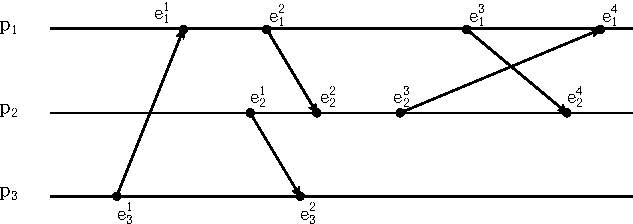
\includegraphics[width=12cm]{2_generic_events.pdf}
    \caption[Beispiel einer beliebigen Kommunikation]{Darstellung einer auf Nachrichten basierten Kommunikation dreier Prozesse. Ereignisse sind als schwarze Punkte auf den Zeitstrahlen und Nachrichten als Pfeile dargestellt.}
    \label{fig:genericEvents}
\end{figure}

Außerdem geht unser Modell davon aus, dass ein Prozess aus drei Schichten besteht.
Dies ist für die theoretische Definition unwesentlich, erleichtert aber die praktische Umsetzung und verbessert das Verständnis.
Die höchste Schicht ist die Anwendungsschicht, hier wird die Applikationslogik implementiert die durch das verteilte System abgebildet werden soll.
In der mittleren Schicht wird die Synchronisation der Kommunikation vorgenommen und kann somit für die Anwendungsschicht transparent  erfolgen.
Die unterste Schicht stellt die Netzwerkschicht dar, die Aufgabe dieser Schicht ist es die Nachrichten physikalisch zu übertragen.

\subsection{Kausalität und Ordnung}
\label{cap:ordnung}
% ungeordnet
% kausale Ordnung
% partielle kausale Ordnung
% totale Ordnung
Die meisten Menschen würden wahrscheinlich sagen, dass ein Ereigniss $a$ vor einem Ereigniss $b$ passierte, wenn $a$ zu einem früheren Zeitpunkt als $b$ auftrat.
Das Konzept \qq{Zeit} ist fundamental in unserer Art zu denken verankert.
Es ist von dem grundlegenderen Konzept der Ordnung in der Ereignisse eintreten abgeleitet.
Die zeitliche Ordnung von Ereignissen bestimmt die Art wie wir über die Funktionsweise Systeme denken \cite{Lamport1978}.

Dies führt zu Überlegungen über den Zusammenhang von Ursache und Wirkung.
Die Verbindung zwischen dem auslösenden Ereignis und dem ausgelösten Ereignis wird als Kausalität bezeichnet.
Es wird also die Abfolge von aufeinander bezogenen Ereignisse oder Zustände betrachtet.
Meist ist es nicht direkt ersichtlich ob Ereignisse kausal zusammenhängen, hierzu müssen die Gegebenheiten und Zusammenhänge der Ereignisse genau bekannt sein.
Dies ist nicht immer gegeben und auch nicht einfach entscheidbar, da hierzu Zusammenhänge betrachtet werden müssen, die meist in einer höhreren Schicht gegeben sind oder schlichtweg für einen Computer.
Daher wird im folgenden immer von potentieller Kausalität gesprochen.
Das bedeutet, dass nur Aussagen darüber gemacht werden ob ein Ereignis die Ursache für ein Anderes sein kann.

In einem einzelnen nicht nebenläufigen Prozess ist die potentielle Kausalität gegeben durch den Programmablauf.
Da die Instruktionen eines Programmes nacheinander ohne Vergabelungen ausgeführt werden und dabei jede Instruktion atomar ist, kann der aktuelle Zustand nur aus den davor ausgeführten Instruktionen bestimmt worden sein.
Hierbei kann eine Instruktion analog zu einem Ereignis verstanden werden.

Im Vergleich hierzu ist die Situation in einem verteilten System oder nebenläufigen Prozess deutlich komplexer.
Durch die Verteilung und Parallelität des Programmcodes ist die \qq{natürliche} Ordnung nicht mehr gegeben.
Innerhalb eines Prozesses ist die Ordnung weiterhin gegeben, da sich ein lokaler Prozess wie oben geschildert verhält.
Wird nun aber das Gesamtbild, also das ganze System betrachtet, sind die Eigenschaften von oben nicht mehr gegeben.
Das Wissen um die Kausalität der Ereignisse ist jedoch häufig notwendig um die Konsistenz des Systems zu wahren.

Der potentielle kausale Zusammenhang zwischen Ereignisse kann durch die Zeit festgestellt werden.
Ein Ereignis, welches zu einem späteren Zeitpunkt eingetreten ist, kann unmöglich die Ursache für ein vorhergehendes Ereignis sein.
Sind also die Zeitpunkte der Ereignisse bekannt, kann eine Aussage über die Kausalität getroffen werden.
Menschen haben ein intuitives Verständnis solcher Zusammenhänge.

Eine zeitliche Ordnung der Ereignisse ist somit die Grundlage für die Erkennung kausaler Zusammenhänge.
Ein Computer hat natürlich kein intuitives Verständnis von Zeit.
Daher müssen einige mathematische Definitionen festgelegt werden, welche die Grundlage für die Implementierung der zeitlichen Ordnungen dienen.

Damit eine Ordnung hergestellt werden kann, müssen die Ereignisse in Relation gesetzt werden können.
Eine Relation wurde bereits beschrieben, nämlich die \qq{Programmordnung} $\rightarrow$.
Lamport \cite{Lamport1978} definiert in seiner Arbeit die \qq{happend before}-Relation $\Rightarrow$ und stellt die kleinste Relation dar, die folgende Bedingungen erfüllt:
\begin{itemize}
    \item Wenn $e_i^x \rightarrow e_i^y$, dann $e_i^x \Rightarrow e_i^y$.
    \item Wenn $e_i^x$ ein Senden Ereignis ist und $e_j^y$ das Empfangen Ereignis der selben Nachricht darstellt, dann folgt $e_i^x \Rightarrow e_j^y$.
    \item Wenn $e_i^x \Rightarrow e_j^y$ und $e_j^y \Rightarrow e_k^z$, dann $e_i^x \Rightarrow e_k^z$.
\end{itemize}

Aus der ersten Bedingung ist ersichtlich, dass aus der strengeren Programmordnung direkt die \qq{happend before}-Relation für zwei lokale Ereignisse abgeleitet werden kann.
Die zweite Bedingung fordert, dass das Empfang Ereignis einer Nachricht nie vor dem Senden Ereignis eintreten kann.
Offensichtlich kann also eine Nachricht nicht empfangen werden, wenn sie noch nicht verschickt wurde.
Dieser Zusammenhang ist für Menschen zwar intuitiv ersichtlich kann nun aber auch für Computer korrekt formuliert werden.
Durch die dritte Bedingung ist die Transitivität der Relation gegeben.
Wurde ein Ereignis $z$ nach $y$ ausgelöst und $x$ vor $y$ gilt logischerweise, dass $x$ auch vor $z$ ausgelöst werden musste und somit $x\Rightarrow z$ gilt.

Ein Ereignis $e_j^y$ gilt als kausal abhängig von $e_i^x$ wenn $e_i^x \Rightarrow e_j^y$, da es nur ausgeführt werden kann wenn die Ausführung von $e_i^x$ bereits abgeschlossen ist.
Alternativ kann $e_i^x$ als Vorbedingung von $e_j^y$ betrachtet werden.

Zwei Ereignisse gelten als gleichzeitig aufgetreten wenn $e_i^x \centernot\Rightarrow e_j^y$ und $e_j^y \centernot\Rightarrow e_i^x$ gilt.
Dann können diese beiden Ereignisse parallel ausgeführt werden, da keines das jeweils Andere kausal beeinflussen kann.
Diese Nebenläufigkeit wird in Symbolen als $e_i^x \parallel e_j^y$ geschrieben.

Es ist offensichtlich, dass jede korrekte logische Uhr die \qq{happend before}-Relation einhalten muss.
Lamport folgert daraus die Uhrbedingung (engl. \qq{clock condition}) die von jeder korrekten logischen Uhr erfüllen muss \cite{Lamport1978}:
\begin{equation*}
\forall e_i^x, e_j^y \in E \colon \text{wenn } e_i^x \Rightarrow e_j^y \text{ dann } C(e_i^x) < C(e_j^y)
\end{equation*}

In Worte gefasst bedeutet diese Bedingung, dass die Uhren zweier Ereignisse durch die kleiner-als-Relation die kausale happend-before-Relation bestimmen.
Der Größenvergleich der Uhren gibt also Aufschluss über die kausale Abhängigkeit der Ereignisse.
Aus dieser Uhrbedingung lassen sich zwei konkrete Bedingungen an den Uhren ableiten, welche sich direkt aus der Definition der $\Rightarrow$-Relation ergeben:
\begin{itemize}
    \item Wenn $e_i^x \rightarrow e_i^y$, dann $C(e_i^x) < C(e_i^y)$.
    \item Wenn $e_i^x$ ein Senden Ereignis ist und $e_j^y$ das Empfangen Ereignis der selben Nachricht darstellt, dann folgt $C(e_i^x) < C(e_i^y)$.
\end{itemize}

Die dritte Bedingung aus der Definition der \qq{happend before}-Relation muss hier nicht explizit wiederholt werden, da diese lediglich die Transitivität beschreibt und diese durch die $<$-Relation der Uhren gegeben ist.

Die eingeführten Regeln erlauben es nun die Zusammenhänge zwischen Ereignisse genauer zu betrachten.
Zustellungsregeln (engl. \qq{delivery rules}) definieren Einschränkungen an der Reihenfolge wie eingehende Nachrichten an den zu verarbeiteten Prozess verschickt werden dürfen.
Eine wichtige Regel ist die FIFO-Zustellung (\qq{First In First Out}) die besagt, dass ein Prozess $j$ Nachrichten in der Reihenfolge empfangen muss wie sie von $i$ aus gesendet wurden.
Dabei können Nachrichten von anderen Prozessen in beliebiger Reihenfolge versandt werden.
Es gilt somit
\begin{equation*}
    \text{wenn } e_i^s \rightarrow e_i^S \text{ dann } e_j^r \rightarrow e_j^R,
\end{equation*}
wobei $s$ und $S$ Sende-Ereignisse darstellen und $r/R$ die entsprechenden Empfang-Ereignisse sind.
In dieser Definition ist keine bestimmte Reihenfolge an Ereignisse von anderen Prozessen gefordert.

Eine weitere, im Vergleich zur FIFO-Zustellung strengere, Zustellungsregel ist die kausale Zustellung (engl. \qq{causal delivery}). Diese ist gegeben 
\begin{equation*}
    \text{wenn } e_i^s \Rightarrow e_k^S \text{ dann } e_j^r \rightarrow e_j^R.
\end{equation*}

Kausale Zustellung erweitert die FIFO-Zustellung um die Einschränkung, dass gesendete Nachrichten von verschiedenen Prozessen geordnet werden, sofern diese kausal nach der \qq{happend before}-Relation zusammenhängen.

Damit ein kausale Zustellung implementiert werden kann, muss die Uhr in der Lage sein Aussetzer in der Kommunikation zu erkennen.
Diese Eigenschaft wird Unterbrechungserkennung (engl. \qq{gap detection}) genannt.
Sie beschreibt den Umstand, dass ein Prozess in der Lage sein muss anhand zweier eingehender Nachrichten und deren Zeitstempel erkennen können muss, dass eine Nachricht existiert die in der Reihenfolge zwischen den beiden vorhanden Nachrichten gehört und bisher nicht empfangen wurde.
Formell gesprochen muss für zwei gegebenen Uhren $C_i(e_i^x) < C_j(e_j^y)$ entschieden werden, ob ein Ereignis $e_k^z$ mit $C_i(e_i^x)<C_k(e_k^z)<C_j(e_j^y)$ existiert \cite{babaoglu1993consistent}.

\subsection{Uhren}
In diesem Kapitel werden unterschiedliche Uhrtypen vorgestellt.
Generell wird zwischen physikalischen und logischen Uhren unterschieden \cite{Tanenbaum2007}.
Die im vorherigen Abschnitt beschrieben Zusammenhänge ermöglichen es logische Uhren formell zu definieren.
Bevor jedoch logische Uhren genauer beschrieben werden, wird zu erst auf physikalische Uhren eingegangen um den Unterschied zu logischen Uhren und deren Motivation zu verdeutlichen.

\subsubsection{Physikalische Uhren}
In der Regel besitzen heutige CPUs Schaltkreise die als Zeitgeber für die Uhrzeit verwendet werden.
Obwohl häufig als Uhr bezeichnet handelt es sich hierbei viel mehr um einen Zähler.
Ein im Prozessor integrierter Quarzkristall schwingt bei angelegter Spannung mit einer fest definierten Frequenz.
Mit dieser gegeben Frequenz kann nun ein Zähler pro Sekunde einmal inkrementiert werden und somit als Zeitgeber verwendet werden.

Bisher wurde die Darstellung eines Zeitpunktes weitestgehend ignoriert. Es liegt nahe, dass die für Menschen intuitive aufgeteilte Darstellung von Datum und Uhrzeit für Computer umständlich ist. Daher gibt es unterschiedliche Systeme, wie ein Zeitpunkt dargestellt werden kann.

Ein gängiges System um Zeitpunkte zu bestimmen ist die Unixzeit.
Dabei werden alle Sekunden seit dem 1. Januar 1970 um 00:00:00 Uhr UTC gezählt.
Ein Zeitpunkt kann daher einfach als Ganzzahl dargestellt werden.
Der große Vorteil dieses Systems liegt in seiner Einfachheit.
So kann mit einer Rechenoperation die Zeitdauer zwischen zwei Timestampes berechnen oder durch einen einfachen Vergleich festgestellt werden, welcher Timestamp weiter in der Vergangenheit liegt.

Wird nun jedem Ereignis in einem verteilten System ein Unix-Timestamp zugewiesen, kann theoretisch eine zeitliche Ordnung der Ereignisse über Prozessgrenze hinaus erreicht werden. Dies wird durch eine einfache Sortierung nach dem Zeitstempel erzielt.
Ein Problem dieser Herangehensweise ist die Auflösung des Zeitstempels. Treten mehrere Ereignisse innerhalb einer Sekunde auf, kann ihre Reihenfolge nicht am Timestamp festgestellt werden, da sich dieser logischerweise nur jede Sekunde ändert.

Hier ist die Unixzeit nicht mehr ausreichend und eine genauere Darstellung muss gewählt werden.
Dabei steigt jedoch die Komplexität bei der Verarbeitung der Zeitstempel.
Zusätzlich ist nicht sofort klar, welche Darstellung als genau genug gilt.
Je kleiner der zeitliche Unterschied zwischen zwei Zeitstempeln desto genauer das System.
Hierbei muss ein Kompromiss zwischen Genauigkeit, Speicherbedarf und Verarbeitungsaufwand gefunden werden.

Ein weiteres Problem von physikalischen Uhren ist ihre Abweichung von der tatsächlichen Zeit.
So besitzt jeder Quartzkristall eine gewisse Schwankung in seiner Frequenz.
Dadurch driftet die Computeruhr immer weiter von der tatsächlichen Zeit ab \cite{Coulouris2011}[S. 598].
Umgangssprachlich würde man sagen, die Uhr geht vor bzw. nach.
Dieses Abdriften lässt sich nur durch Verwendung von genaueren Uhren wie z.B. Atomuhren vermeiden.
Es ist jedoch unpraktikabel in jeden Computer eine Atomuhr zu installieren, daher muss die Uhr eines Computers mit einer anderen exakten Uhr regelmäßig synchronisiert werden.
In Netzwerken wird hierzu in der Regel das in der Einleitung erwähnte Network Time Protocol verwendet \cite{Coulouris2011}[S. 603].

Dieser Abweichung einzelner Uhren kann durch geeigneter Algorithmen entgegnet werden.
Ein solcher Algorithmus ist der Berkeley-Algorithmus \cite{gusella1989accuracy}. 
Dieser erfordert jedoch einen globalen Zeitgeber, der im Gegensatz zu NTP, aktiv die Zeit im Netzwerk verteilt.
Im Allgemeinen wird in verteilten Systemen davon ausgegangen, dass keine globale Uhr existiert und somit physikalische Uhren nicht zur Anwendung kommen \cite{Tanenbaum2007}[S. 11].

Für ein verteiltes System kann der absolute Fehler einer Uhr vernachlässigt werden, solang alle beteiligten Prozesse den selben Fehler haben und somit relativ innerhalb des Systems richtig sind.
Liegen zum Beispiel die Uhren aller Prozesse exakt 10 Sekunden in der Vergangenheit, kann die Reihenfolge der Ereignisse immer noch festgestellt werden. 
Weisen jedoch nur manche Prozesse einen Fehler auf, kann die Reihenfolge nicht mehr korrekt aus den Zeitstempel erschlossen werden.
Ist die Zeit aller Prozesse System intern konsistent, kann auf eine Synchronisation einer externen realen Zeit verzichtet werden \cite{bengel2015masterkurs}[S. 359].
Diese Überlegung führt zu der Definition von logischen Uhren.

\subsubsection{Lamport-Uhren}
\label{cap:vectorclock}
Leslie Lamport beschreibt in seinem Paper \cite{Lamport1978}, indem er gleichzeitig kausale Ordnung definiert, ein Verfahren um Prozesse durch logische Uhren zu synchronisieren.
Sein vorgeschlagener Algorithmus ist heute als Lamport Uhr bekannt und stellt eine simple Möglichkeit dar, partielle kausale Ordnung in einem verteilen System herzustellen.
Lamport führt den Begriff der logischen Zeit ein.
Hierbei verläuft die logische Zeit diskret und schreitet nur voran, wenn ein Ereignis eintritt \cite{leon2013ereignisdiskrete}.
Eine logische Uhr erfasst die logische Zeit indem bei eintritt eines Ereignisses ein Zähler inkrementiert wird.
Dabei hält jeder Prozess einen eigenen Zähler.
Sendet nun ein Prozess eine Nachricht, hängt er seinen aktuellen Zählerstand als Zeitstempel an die Nachricht an.
Empfängt nun ein anderer Prozess eine Nachricht kann er anhand des Zeitstempels der Nachricht und seiner lokalen Uhr den kausalen Zusammenhang erschließen.

Formal ist eine Lamportuhr $C$, wie alle logische Uhren, als eine Funktion definiert, welche einem Ereignis $e$ eine Nummer $C(e)$ zuweist.
Lamport Uhren erfüllen die Uhrbedinung aus Abschnitt~\ref{cap:ordnung}, indem jeder Prozess $i$ seine eigene Uhr $C_i$ hält und nach folgenden Regel aktualisiert:
\begin{itemize}
    \item Wenn $e_i^x$ kein Empfang-Ereignis ist, dann ist $C_i(e_i^x):=C_i(e_i^{x-1})+1$
    \item Ist $e_i^x$ ein Empfang-Ereignis der Nachricht $m$, dann ist $C_i(e_i^x):=\max\{C_i(e_i^{x-1}), C_j(e_j^y)  \} + 1$, wobei Prozess $j$ die Nachricht $m$ an $i$ geschickt hat und $C_j(e_j^y)$ der Uhrwert des Sende-Ereignis ist.
\end{itemize}

\fig{fig:lamportBsp} zeigt eine exemplarische Kommunikation zwischen drei Prozessen, dabei wird die Lamportuhr zum Zeitpunkt eines Ereignisses als Zahl in der Grafik dargestellt.
Es ist einfach zu zeigen, dass Lamportuhren die Uhrbedingung erfüllen.
Hierbei muss gezeigt werden, dass die aus der Uhrbedingung abgeleiteten Bedingungen erfüllt sind.
Wird eine Nachricht versendet, muss die lokale Lamportuhr inkrementiert werden. 
Daraus folgt, dass für zwei direkt aufeinander folgenden Sende-Ereignisse $e_i^x$ und $e_i^y$ wobei $e_i^x \rightarrow e_i^y$ gilt $C(e_i^x) < C(e_i^y)$, da bei Eintritt von $e_i^x$ die Uhr auf $a$ inkrementiert wurde und bei $e_i^y$ auf $a + 1$ erhöht werden musste.

\begin{figure}[ht]
    \centering
    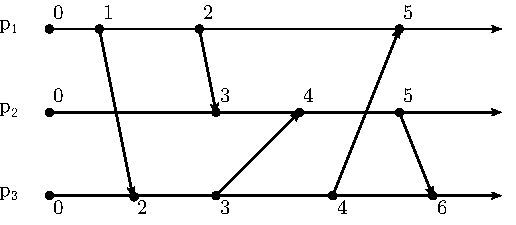
\includegraphics[width=0.80\textwidth]{LamportBeispiel.pdf}
    \caption[Exemplarische Kommunikation mit Lamport Uhr]{Kommunikation zwischen drei Prozessen unter Verwendung von Lamportuhren.}
    Nachgezeichnet aus  \cite{landes2006dynamic}
    \label{fig:lamportBsp}
\end{figure}

Die zweite Bedingung fordert, dass für ein Sende-Ereignis $e_i^x$ die Uhr einen kleineren Wert als die des entsprechenden Empfangs-Ereignis $e_j^y$ besitzt.
Durch die $\max$-Funktion wird zwischen der lokalen Uhr und der an die Nachricht angehängte Uhr entschieden.
Hieraus entstehen zwei Fälle:
Im ersten Fall ist der Zähler der lokalen Uhr größer als die der Nachricht, somit ist die Nachricht älter als der aktuelle Zustand und die lokale Uhr inkrementiert um Eins stellt den neuen Uhrenwert dar.
Im zweiten Fall ist die Uhr der Nachricht größer als die lokale Uhr.
Dem Empfänger sind also nicht alle Ereignisse des Sendeprozesses bekannt und hat somit einen älteren Stand.
In diesem Fall wird die Uhr aus der Nachricht als neue Uhr übernommen und inkrementiert.
In beiden Fällen gibt die Uhr für das Sende-Ereignis immer einen kleineren Wert als für das Empfangs-Ereignis an somit ist $C(e_i^x) < C(e_j^y)$ erfüllt.

Lamportuhren haben jedoch einen entscheidenden Nachteil.
Mit ihnen können keine Unterbrechungen erkannt werden.
Da dies jedoch die Grundlage für kausaler und FIFO-Zustellung ist, sind Lamportuhren nicht dafür geeignet diese zu garantieren.
Der Grund hierfür ist, dass keine Information über den Zustand der anderen Prozesse gespeichert wird.

Haben zwei Ereignisse den selben Zählerstand müssen diese gleichzeitig aufgetreten sein.
Ist also $C_i(e_i^x)=C_j(e_j^y)$ gegeben, folgt $e_i^x \parallel e_j^y$.
Gilt jedoch $C_i(e_i^x)<C_j(e_j^y)$ ist es nicht möglich zu entscheiden ob $e_i^x \Rightarrow e_j^y$ oder $e_i^x \parallel e_j^y$ gilt.
Die Uhr erlaubt es also nicht eine Aussage über die Reihenfolge der Ereignisse selbst zu machen.

Lamportuhren sind dazu geeignet eine totale Ordnung im System herzustellen.
Diese strikte Ordnung muss jedoch mit einer großen Anzahl an verschickten Nachrichten bezahlt werden, was wieder eine hohe Netzwerklast mit sich bringt.
Es würde daher ausreichen, Ereignisse nach ihrem kausalen Zusammenhang zu ordnen.
\fig{fig:LamportConcurrent} zeigt eine solche Situation, in der eine kausale Ordnung ausreichen würde, da das Empfangen von Nachricht $m_2$ nicht davon abhängt ob $m_2$ bereits empfangen wurde.
Eine totale Ordnung würde jedoch dazu führen, dass $m_1$ und $m_2$ von jedem Prozess in der selben Reihenfolge empfangen werden.
Ferner ist es nicht möglich ob das Versenden von $m_3$ vom Empfangen von $m_1$ oder $m_2$ abhängt \cite{Tanenbaum2007}.

\begin{figure}[ht]
    \centering
    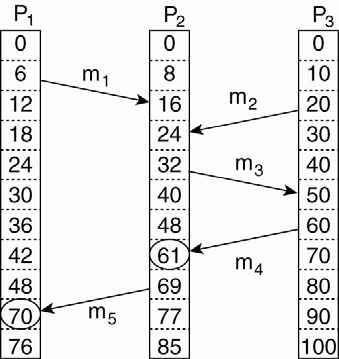
\includegraphics[width=0.40\textwidth]{LamportConcurrent.png}
    \caption[Lamportuhren und Kausalität]{Nebenläufige Nachrichtenübertragung unter Verwendung von Lamportuhren.}
    Quelle: \cite{Tanenbaum2007}
    \label{fig:LamportConcurrent}
\end{figure}

Mit Lamportuhren können Ereignisse somit nach ihren kausalen Abhängigkeiten geordnet werden.
Es kann jedoch keine Aussage über die Abhängigkeiten selbst getroffen werden.
So kann zum Beispiel nicht entschieden werden ob zwei Ereignisse in der kausalen Ordnung vertauscht werden können ohne die kausale Konsistenz zu zerstören.
Hierzu müssen zusätzliche Informationen über die restlichen Prozesse gespeichert werden.

% negativ Beispiel in Plausible Clocks Constant Size Logical Clocks for Distributed Systems
\subsubsection{Vektoruhren}
Vektoruhren stellen eine Erweiterung der von Lamport vorgestellten Uhr dar und werden häufig eingesetzt um die Defizite der Lamportuhr zu beheben.
Statt einem einzelnen skalaren Zeitstempel, verwenden Vektoruhren viele Zähler um die kausale Abhängigkeit zwischen Ereignisse umfänglicher zu erfassen, als dies mit Lamportuhren möglich wäre.
Ihr Name wurde ihnen gegeben, da die Zeitstempel in einem Vektor zusammengefasst werden.
Sie wurden zeitgleich von Mattern \cite{mattern1989virtual} und Fidge \cite{fidge1991logical, fidge1988timestamps} vorgeschlagen und analysiert.

Wie bei Lamportuhren verwaltet jeder Prozess seine eigne lokale Uhr.
Die Uhr ist jedoch nun ein Vektor aus $n$ skalaren Werten, bei einem System bestehend aus $n$ Prozesse.
Jede Komponente $VC_i(e_i^x)[j]$ entspricht dem letzten Uhrenwert den Prozess $i$ zu Prozess $j$ zum Zeitpunkt $e_i^x$ kennt.
Folgende Regeln müssen bei der Aktualisierung der Uhr eingehalten werden:
\begin{itemize}
    \item Wenn $e_i^x$ das Empfang-Ereignis der Nachricht $m$ ist, dann $VC_i(e_i^x):=\max\{ VC_i(e_i^{x-1}), VC_j(e_j^y) \}$, wobei $VC_j(e_j^y)$ der Uhrenvektor des Sende-Ereignisses von Prozess $j$ ist, welcher die Nachricht $m$ an Prozess $i$ gesendet hat. Das Maximum wird komponentenweise bestimmt.
    \item Wenn $e_i^x$ ein beliebiges Ereignis ist, dann muss der Prozess seine Vektorkomponente inkrementiert: $VC_i(e_i^x)[i]:=VC_i(e_i^{x-1})[i] + 1$. Dies beinhaltet auch Empfang-Ereignisse.
\end{itemize}

\fig{fig:VektorBsp} zeigt den selben Kommunikationsverlauf wie \fig{fig:lamportBsp} jedoch mit der Verwendung von Vektoruhren statt Lamportuhren.
Anschaulich betrachtet ist $\VCieix[i]$ gleich der Anzahl der von Prozess $i$ ausgeführten Ereignisse (inklusive $\eix$) zum Zeitpunkt von $\eix$ bereits ausgeführt hat.
Nach der selben Logik gibt $\VCieix[j]$ die Anzahl der Ereignisse von Prozess $i$ an, die vor $\eix$ eingetreten sind.

\begin{figure}[ht]
    \centering
    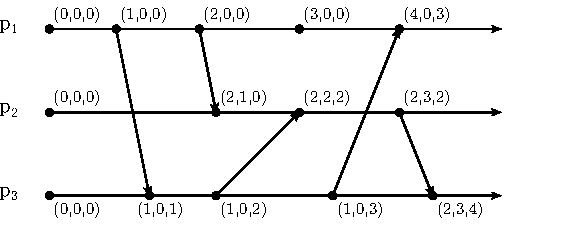
\includegraphics[width=0.80\textwidth]{VektorBeispiel.pdf}
    \caption[Exemplarische Kommunikation mit Vektoruhren]{Kommunikation zwischen drei Prozessen unter Verwendung von Vektoruhren.}
    Nachgezeichnet aus  \cite{landes2006dynamic}
    \label{fig:VektorBsp}
\end{figure}

Der große Vorteil von Vektoruhren ist, dass sie nicht nur die schwache Uhrenbedingung erfüllen sondern auch eine strengere Variation, nämlich die starke Uhrenbedingung \cite{Lamport1978}:
\begin{equation*}
\forall e_i^x, e_j^y \in E \colon VC(e_i^x) < VC(e_j^y) \text{ genau dann, wenn } e_i^x \Rightarrow e_j^y
\end{equation*}

Bei Lamportuhren, welche nur die schwache Uhrenbedingung erfüllen, ist die Aussage $C_i(e_i^x)<C_j(e_j^y)$ doppeldeutig. 
Es kann nicht zwischen $e_i^x \Rightarrow e_j^y$ oder $e_i^x \parallel e_j^y$ unterschieden werden.
Bei Uhren die jedoch die starke Uhrenbedingung erfüllen, wie Vektoruhren, lässt die selbe Aussage nur den Schluss zu, dass $e_i^x \Rightarrow e_j^y$ gelten muss.
Somit wurde die Schwäche von Lamportuhren eliminiert.

Damit die starke Uhrenbedingung von Vektoruhren erfüllt werden kann, muss zuerst die $<$-Relation von Vektoruhren definiert werden:
\begin{align*}
\VCieix &< \VCjejy \text{ genau dann, wenn} \\
       & \VCieix \ne \VCjejy \text{ und } \\
       & \forall k | 1 \leq k \leq n \colon \VCieix[k] \leq \VCjejy[k].
\end{align*}

Nun kann anhand einer Vektoruhr entscheiden werden ob ein Ereignis kausal abhängig von einem Anderen ist:
\begin{equation*}
    \eix \Rightarrow \ejy \text{ genau dann, wenn } \VCieix[i] \leq \VCjejy[i].
\end{equation*}

Hervorzuheben ist, dass nur eine einzige skalare Operation notwendig ist, um diesen Zusammenhang zu erschließen.
Ferner ist die obige Formel nicht symmetrisch.
Wird sie angewendet und ergibt $\eix \centernot\Rightarrow \ejy$, muss sie ein zweites Mal angewendet werden um zwischen $\ejy \Rightarrow \eix$ oder $\eix \parallel \ejy$ zu entscheiden.
Dies führt zu dem Nebenläufigkeitstest:
\begin{align*}
    \eix \parallel & \ejy \text{ genau dann, wenn } \\
                   & \VCjejy[i] \le \VCieix[i] \text{ und } \\
                   & \VCieix[j] \le \VCjejy[j].
\end{align*}

Ergibt der Test $\eix \centernot\parallel \ejy$ kann direkt anhand des nicht erfüllten Terms der beiden Bedingungen entschieden werden ob $\eix \Rightarrow \ejy$ oder $\ejy \Rightarrow \eix$ gilt.

Der große Nachteil von Vektoruhren besteht darin, dass ein fixer Index verwendet wird, um die Komponenten im Vektor auszuwählen die den skalaren Uhrenwert eines Prozesses darstellt.
Dies führt zu zwei sehr einschränkenden Voraussetzungen.
Zum einen muss die Anzahl der Prozesse konstant und zum anderen auch im Voraus bekannt sein.
In dynamischen System stellen diese beiden Einschränkungen ein ernstes Problem dar, da die Anzahl in solchen System nicht einfach zu bestimmen ist, was in der Natur der Sache liegt \cite{landes2006dynamic}.

\subsubsection{Interval Tree Clocks}
Vektoruhren haben den großen Nachteil für dynamischen Systeme eher ungeeignet zu sein.
Daher ist es interessant entsprechende neue Verfahren zu untersuchen, welche die Defizite von Vektoruhren in einem solchen Kontext ausmerzen.
Interval Tree Clocks (ITC) stellen ein solches Verfahren dar und wurden 2008 von \etal{Almeida} in ihrer Arbeit \qq{Interval Tree Clocks: A Logical Clock for Dynamic Systems} \cite{almeida2008treeclocks} vorgeschlagen.
Wie bereits angedeutet, sind ITCs besonders für dynamische Systeme geeignet, in denen häufig Prozesse gestartet und terminiert werden.
Während Vektoruhren eine globale ID benötigen, nämlich den Index der Vektorkomponente, kommen ITCs ohne solcher globalen eindeutigen IDs aus. Dies ermöglicht eine gänzlich dezentrale Erzeugung von Prozessen \cite{almeida2008treeclocks}.

Interval Tree Clocks haben eine in der Größe variable Darstellung, welche sich automatisch an der Anzahl der existierenden Prozesse richtet. Die Größe der Uhren nimmt zu und ab entsprechend der im System aktiven Prozesse.
Um dies zu erreichen setzten ITCs auf dem \qq{Fork-Event-Join}-Modell auf.
Hierbei handelt es sich um ein Modell bei dem die Kausalität durch drei grundlegende Operationen beschrieben werden kann.
Diese Operationen, fork, event und join, werden auf die Zeitstempel der Uhr angewendet.
Bei ITCs besteht ein Zeitstempel aus dem Paar $(i,e)$ bestehend aus einer ID $i$ und der Ereigniskomponente $e$, welche die kausal bekannte Ereignisse enthält.

Durch die fork-Operation kann die vergangenen kausale Zusammenhänge eines Zeitstempel geklont werden.
Dies führt dazu, dass zwei neue Paare entstehen mit der selben Ereigniskomponente, jedoch mit unterschiedlichen IDs.
Neue Ereignisse können durch die event-Operation zu der Ereigniskomponente hinzugefügt werden. 
Hierbei wird die partielle Ordnung der Ereignisse eingehalten.
Mit der join-Operation kann ein neuer Zeitstempel durch Zusammenfassung zweier Stempel erzeugt werden.

Mit diesen Basisoperationen lassen sich nun die klassischen Operationen send, receive und sync beschreiben.
Eine send-Operation ist die atomare Verkettung von event und fork.
Bei Vektoruhren entspricht dies dem Inkrementieren des lokalen Zählers und dem erzeugen einer Nachricht.
Receive wird ebenfalls durch die atomare Verkettung von join gefolgt von event beschrieben.
Analog hierzu muss bei Vektoruhren das komponentenweise Maximum bestimmt werden und der lokale Zähler inkrementiert werden.
Wieder durch eine atomare Verkettung kann die sync-Operation durch join und fork modelliert werden.

Der Unterschied zwischen Vektoruhren und ITCs wird besonders deutlich, wenn die IDs als Funktion betrachtet werden.
Während die global eindeutige IDs von Vektoruhren einer konstanten vordefinierten Funktion entspricht, wird die ID Komponente der ITCs entsprechend der Prozessanzahl modifiziert.
Während bei klassischen Verfahren diskrete Funktionen verwendet werden, basieren ITCs auf kontinuierliche Funktionen über die Menge $\mathbb{R}$, beschränkt auf das Intervall $[0;1[$.
Dieser Bereich kann in eine beliebige Anzahl an Subintervallen geteilt werden.

Die Idee hinter Interval Tree Clocks ist es nun jedem Prozess eine Menge von Intervalle zur Verfügung zustellen, welche verwendet werden können um die Ereigniskomponente zu erweitern.
Diese werden bei einer fork-Operation an die beiden Nachfolger weitergegeben und bei einer join-Operation wieder zusammengeführt.
Jedes Subintervall wird durch aufeinanderfolgend Teilungen des Intervalls $[0;1[$ in gleich große Intervalle erzeugt.
Diese Zusammenhänge lassen sich effizient als binärer Baum darstellen.
\etal{Almeida} stellen eine geeignete binäre Kodierung der ITCs in ihrer Arbeit vor \cite{almeida2008treeclocks}.

\fig{fig:itcBsp} zeigt die Veränderung der ITCs im Laufe der Zeit unter Verwendung des Fork-Join-Event-Modell.
Die Kommunikation, im dargestellten Beispiel, beginnt mit einem Prozesse, welcher einen \qq{Seed}-Zeitstempel hält.
ITCs lassen sich als Funktion beschreiben und somit plotten.
Die in der Grafik zu sehende Rechtecke stellen die Graphen der ITCs Funktionen dar.
Dieser wird in zwei Uhren geteilt, es sind nun zwei Prozesse aktiv.
Für einen der beide Prozesse wird ein Ereignis ausgelöst, für den Anderen zwei.
Dies ist durch die Stapelung der Graphen angedeutet.
Nun wird wieder ein fork ausgeführt. Dies führt dazu, dass drei Prozesse aktiv sind.
Anschließend werden zwei Prozesse zusammenführt, um anschließend direkt wieder geteilt zu werden.
Zum Ende werden zwei Prozesse wieder zusammengeführt.

Interval Tree Clocks können somit effizienter in dynamische Systeme verwaltet werden, als zum Beispiel Vektoruhren.
Sie wurden im Hinblick auf die häufige Erstellung und Terminierung von Prozessen, wie es in heutigen Systemen in der Regel der Fall ist, entwickelt.
Dabei wird der dynamische Charakter solcher Systeme in der dynamischen Aufteilung der Intervalle der ITCs widergespiegelt.
Fernen kann auf globale eindeutige IDs verzichtet werden, was im Allgemeinen eine große Vereinfachung des Systems darstellt.

\begin{figure}[ht]
    \centering
    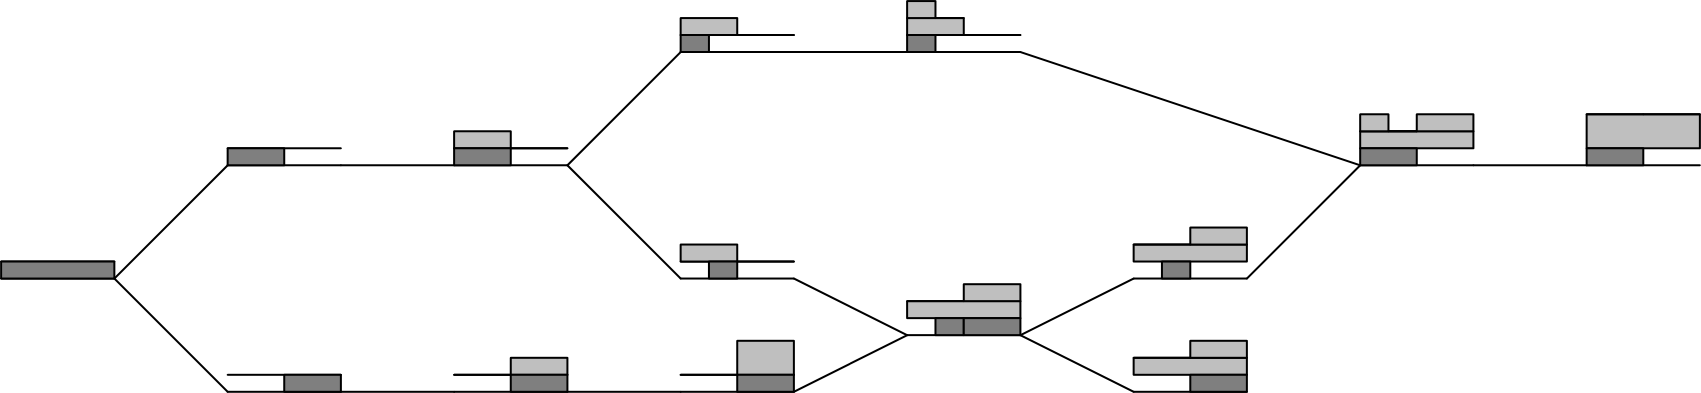
\includegraphics[width=1\textwidth]{ITCBeispiel.png}
    \caption[Fork-Join-Event-Modell von Interval Tree Clocks]{Grafische Darstellung des Fork-Join-Event Modells bei Verwendung von Interval Tree Clocks in einem dynamischen System.}
    Quelle: \cite{almeida2008treeclocks}
    \label{fig:itcBsp}
\end{figure} 






\cleardoublepage
\section{Funktionsweise von Vektoruhren}

In diesem Kapitel wird die allgemeine Funktionsweise von Vektoruhren behandelt. Mittels geeigneten Beispielen wird die Kommunikation in einem einfachen verteilten System illustriert, um die Funktionsweise von Vektoruhren innerhalb der Kommunikation zu zeigen. Zuletzt wird auf das System eingegangen, welches im Rahmen dieser Arbeit in der Programmiersprache C\# implementiert wurde.
\subsection{Prinzipielle Funktionsweise}

Wie bereits beschrieben wurde, bilden Vektoruhren eine Erweiterung der Lamportuhr. Dabei wird in jedem Prozess im System ein Integer als Zähler in der Vektoruhr gespeichert. Im Allgemeinen werden durch eine Vektoruhr Zeitstempel mit Events im System assoziiert \cite{Baldoni:2002:FDC:1435723.1437765}[S. 3].

Jeder Prozess im System besitzt seine eigene Vektoruhr in der Form eines Vektors $VC_i[1...n]$, wobei alle Elemente der Uhr mit $0$ initialisiert werden. Die Uhr eines Prozesses wird wie folgt verwaltet und aktualisiert:

\begin{itemize}
	\item[R1]Jedes mal, wenn ein Prozess $P_i$ ein Event auslöst, muss dieser seine Vektoruhr für den Eintrag $VC_i$ um Eins hochzählen, es gilt  $VC_i[i] := VC_i[i] + 1$. Dadurch verdeutlicht der Prozess, dass er etwas getan hat und signalisiert dies den anderen Prozessen durch aktualisieren seiner Vektoruhr 
	\item[R2]Sendet ein Prozess $P_i$ eine Nachricht $m$, so hängt er seine aktuelle Vektoruhr $VC_i$ an die zu sendende Nachricht an. Auf diese Weise gelangt die Uhr zu dem Empfänger der Nachricht.
	\item[R3]Empfängt ein Prozess $P_i$ eine Nachricht, so muss er seine Vektoruhr aktualisieren. Dabei geht er wie folgt vor: $VC_i = \max(VC_i, m.VC)$. Dies bedeutet, dass der Prozess für jedes Element seiner Vektoruhr überprüft ob der Wert in der Uhr der Nachricht größer als der eigene ist. Sollte dies der Fall sein, wird der eigene Wert an dieser Stelle mit dem Wert aus der anderen Uhr überschrieben.\label{R3}
\end{itemize} \cite{Baldoni:2002:FDC:1435723.1437765}[S. 4]

Die Werte innerhalb einer Vektoruhr $VC_i$ haben eine besondere Bedeutung für den Prozess $P_i$. $VC_i[i]$ gibt die Anzahl an Events an, welche $P_i$ zu dem Zeitpunkt des Betrachtens verarbeitet hat. Die anderen Werte der Uhr ($VC_i[j]$ mit $j \neq i$) zeigen an, dass alle Events welche durch den Prozess $P_j$ verarbeitet wurden, sich kausal betrachtet in der Vergangenheit von $P_i$ befinden. Sie geben sozusagen an, was der Prozess $P_i$ über die Zeiten der anderen Prozesse weiß, diese Information kann sich zu dem Zeitpunkt jedoch bereits von den tatsächlichen Zeiten unterscheiden. Da jeder Prozess lediglich seinen Zähler in der Vektoruhr erhöhen darf, hat dieser Prozess zu jedem Zeitpunkt den aktuellsten Stand seiner lokalen Zeit. \cite{SINGHAL199247}[S. 48]

\subsubsection{Vergleich von Vektoruhren untereinander}
\label{vergleich}
Eine Besonderheit der Vektoruhren besteht im Vergleich von Uhren untereinander. Dies wird notwendig, sobald ein Prozess eine Nachricht erhält und diese verarbeiten muss. Wie in Bedingung R3 unter \ref{R3} - \nameref{R3} zu sehen, muss der Prozess seine Uhr entsprechen der mitgeschickten Vektoruhr der Nachricht aktualisieren. Der Vergleich zwischen der eigenen und der empfangenen Uhr muss dann auf Anwendungsebene geschehen, denn dort wird entschieden was mit der angekommenen Nachricht geschieht.

Für zwei zu vergleichende Uhren $VC_1$ und $VC_2$ gibt es folgenden Beziehungen:

\begin{eqnarray}
&VC_1 \leq VC_2& \text{ wenn } \forall i : VC_1[i] \leq VC_2[i] \\
	&VC_1 < VC_2& \text{ wenn } VC_1 \leq VC_2 \text{ \& } VC_1 \neq VC_2 \\
	&VC_1 \mid \mid VC_2& \text{ wenn } !(VC_1 < VC_2) \text{ \& } !(VC_2 < VC_1)
\end{eqnarray}
\cite{Mattern88virtualtime}[S. 127, Definition 4]

Fall (1) bedeutet, dass eine Uhr $VC_1$ kleiner oder gleich $VC_2$ ist, wenn jedes Element von $VC_1$ kleiner oder gleich dem entsprechenden Element in $VC_2$ ist. Der zweite Fall (2) liegt vor, wenn Fall (1) zutrifft und zusätzlich kein Element in $VC_1$ gleich dem entsprechenden Element in $VC_2$ ist. 
Der letzte Fall (3) ist ein Besonderer Fall. Dieser trifft ein wenn nicht entschieden werden kann, welche Uhr neuer oder älter beziehungsweise nach der obigen Definition größer oder kleiner ist als die andere. Die entsprechenden Nachrichten wurden sozusagen gleichzeitig abgeschickt. Dieser im Englischen als \glqq Concurrent\glqq{} bezeichnete Fall stellt ein großes Problem für Systeme dar, die Vektoruhren für die zeitliche Synchronisation der Kommunikation nutzen. Auf diesen Sonderfall wird im nächsten Kapitel genauer eingegangen.

\subsection{Beispiel einer Kommunikation}

Um die Funktionsweise von Vektoruhren genauer zu beschreiben, wird nun zunächst anhand eines einfachen Beispieles die Kommunikation in einem System mit drei Prozessen sowie die Verarbeitung der Vektoruhren eines jeden Prozesses gezeigt.

\subsubsection{Beispiel einer konfliktfreien Kommunikation}

\begin{figure}[ht]
	\centering
	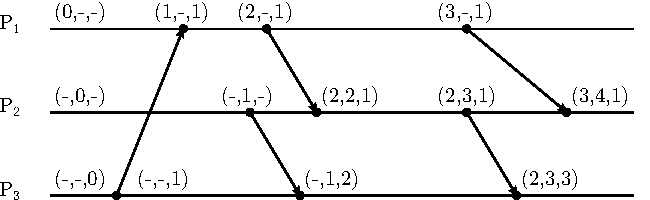
\includegraphics[width=12cm]{KommBeispiel1.pdf}
	\caption[Beispiel einer konfliktfreien Kommunikation]{Ablauf der Kommunikation dreier Prozesse mit Veranschaulichung der dabei auftretenden Vektoruhren.}
	Quelle: Nachgezeichnet aus \cite{Baldoni:2002:FDC:1435723.1437765}
\label{figure:kommBeispiel1}
\end{figure}
\FloatBarrier

Zu Beginn weiß jeder Prozess nur seine lokale Zeit, der Wert $VC_i$ für Prozess $P_i$ wird deshalb auf $0$ gesetzt. Da der Prozess noch keine Kenntnis über die anderen Teilnehmer im System hat, werden die anderen Einträge mit \qq{$-$} initialisiert.

Zu Beginn sendet in dem in Abbildung \ref{figure:kommBeispiel1} abgebildeten Beispiel Prozess $P_3$ eine Nachricht an $P_1$. Er erzeugt dabei ein Event und muss deshalb zunächst seine lokale Vektoruhr inkrementieren, der Wert $VC_3[3]$ wird also um $1$ erhöht. Die Uhr hat nun den Wert \vc{-}{-}{1}. Anschließend wird die lokale Uhr an die zu sendende Nachricht angehängt und diese verschickt.
Nun empfängt Prozess $P_1$ diese Nachricht. Gemäß Regel R1 muss zunächst die lokale Uhr entsprechend der mitgeschickten Uhr aktualisiert werden. Da in jedem Feld der Uhr das Maximum genommen wird, wird die lokale Uhr von $P_1$ nach der Aktualisierung von \vc{0}{-}{-} auf \vc{1}{-}{1} geändert. Da das Empfangen einer Nachricht auch als Event angesehen wird, erhöht sich auch der Wert für den lokalen Zähler von $P_1$ innerhalb der Uhr um $1$.

In diesem Beispiel kommen alle Nachrichten passend nacheinander an und es kann zu keinen Konflikten in der Ausführungsreihenfolge kommen. Das Nachfolgende Beispiel verdeutlicht den Fall, dass Gesendete Nachrichten auch von anderen Nachrichten abhängig und während der Übertragung verzögert ankommen können, was ein Problem eines einfachen Systems mit Vektoruhren darstellt.

\subsubsection{Beispiel einer Kommunikation mit Konflikten}

Das zweite Beispiel lässt sich auf ein verteiltes System anwenden, welches ein Bankensystem mit einem Konto und drei unabhängigen Bankautomaten als Prozesse abbildet. Jeder Automat speichert als Daten den aktuellen Kontostand ab. Wird eine Aktion ausgeführt, zum Beispiel eine Ein- oder Auszahlung, so sendet der Automat per Broadcast eine Nachricht mit der Aktualisierung und seiner Vektoruhr an alle anderen Automaten im System.

\begin{figure}[ht]
	\centering
	\includegraphics[width=12cm]{KommBeispiel2.pdf}
	\caption[Beispiel einer konfliktbehafteten Kommunikation]{Ablauf der Kommunikation in einem Bankensystem, bei dem durch einen Broadcast ein Konflikt beim Vergleich von Vektoruhren auftritt.}
	\label{figure:kommBeispiel2}
\end{figure}
\FloatBarrier

Zu Beginn werden die Vektoruhren der Prozesse wie im vorherigen Beispiel beschrieben initialisiert. Das erste Event passiert an Prozess 2. Hier wird beispielsweise etwas eingezahlt oder abgehoben, die tatsächliche Aktion spielt für das Beispiel weniger eine Rolle als die Tatsache, dass sich etwas an dem Kontostand geändert hat. Der Prozess $P_2$ schickt nun einen Broadcast mit dem aktualisierten Kontostand und seiner lokalen, ebenfalls aktualisierten Uhr an die übrigen Bankautomaten. Diese empfangen die Nachricht und behandeln sie entsprechend.

Der Konflikt passiert in diesem Beispiel bei den nächsten beiden Events. Zunächst wird an Prozess $P_3$ ein Event ausgelöst. Dieser versucht nun, einen Broadcast an die anderen Automaten zu senden, was jedoch aus technischen Gründen fehlschlägt, so dass die Aktualisierungsnachricht nicht bei den übrigen Prozessen ankommt. Zeitgleich zu diesem Event wird auf Automat $P_1$ der Kontostand aktualisiert. Der Prozess sendet nach der Aktualisierung des Kontos sowie seiner lokalen Uhr den Broadcast. Der eigentliche Konflikt entsteht nun an Prozess $P_3$, denn dessen Änderung am Konto ist nicht in das Event von $P_1$ mit eingeflossen, die beiden Aktionen wurden also Zeitgleich ausgeführt und es kann durch Vergleich der Vektoruhren nicht entschieden werden, welches Event von dem anderen stattgefunden hat. Nach den Regeln für den Vergleich von Vektoruhren in Kapitel \ref{vergleich} entspricht dies dem dritten Fall.

Eine Praktische Bedeutung hätte dies, wenn in $P_3$ bei einem Kontostand von 100 \euro{} ein Betrag von 60 \euro{} abgehoben würde. Werden nun zeitgleich an Automat $P_1$ 80 \euro{} abghoben, so hat der Automat $P_3$ nun seine lokalen Kontostand über 20 \euro{} sowie den empfangenen von 40 \euro{}. Ein solcher Konflikt kann nicht durch die Verwendung von Vektoruhren gelöst werden und muss an eine Anwendungsapi weitergereicht werden.  

\subsection{Umsetzung in C\#}
Für die Umsetzung dieses Themas wurde C\# als Programmiersprache ausgewählt. Damit die zeitliche Synchronisation mittels Vektoruhren möglichst realitätsnah simuliert werden kann, wurden drei virtuelle Maschinen mit dem Betriebssystem Windows 8.1 aufgesetzt. Diese befinden sich im Hochschulnetzwerk und können per Remote Desktop bedient werden.

Die Implementierung wurde in zwei unabhängige Programmteile aufgeteilt. Diese sind ein Commander sowie Nodes. 

\begin{figure}[ht]
	\centering
	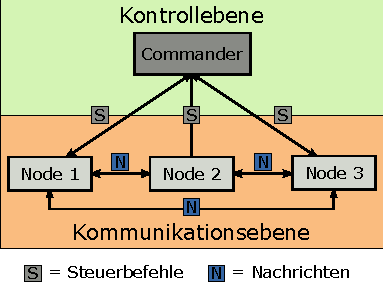
\includegraphics[width=8cm]{CodeAufbau.pdf}
	\caption[Aufbau der Anwendung]{Schematischer Aufbau des implementierten verteilten Systems. Jeder Node ist ein eigenständiger Prozess welcher jeweils auf einer eigenen virtuellen Maschine läuft. Der Kommander wird auf einer der VMs ausgeführt und koodiniert die Kommunikation zwischen den Nodes. Dadurch wird die Kommunikation eines verteilten Systems simuliert.}
	\label{figure:systemaufbau}
\end{figure}
\FloatBarrier

Der Commander stellt sozusagen eine übergeordnete Kommandozentrale dar, welche die Kommunikation der Nodes untereinander durch gewisse Steuerbefehle koordiniert. Er besitzt eine grafische Oberfläche, welche mittels WPF erstellt wurde.

\begin{figure}[ht]
	\centering
	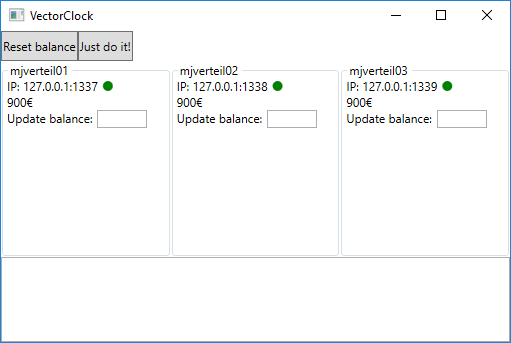
\includegraphics[width=8cm]{commanderWindow.png}
	\caption[Commander Window]{Abbildung des Commanderfensters, welcher dazu dient, die Kommunikation zwischen den Nodes durch Steuerbefehle zu koordinieren}
	\label{figure:commanderWindow}
\end{figure}
\FloatBarrier

Ein Node stellt einen Prozess in dem simulierten System dar. In diesem werden Events ausgeführt und Vektoruhren verarbeitet. Jeder Node besitzt seine eigene, lokale Vektoruhr. Bei einem Node handelt es sich um ein Kommandozeilenprogramm, welches auf einer VM läuft und ständig auf Nachrichten wartet. Damit der Ablauf der Kommunikation besser nachvollzogen werden kann, gibt ein Node bei jedem Event die Details der Nachricht sowie seiner Vektoruhr aus. Zusätzlich sendet er dabei eine Antwort an den Commander mit der Nachricht, welche er erhalten hat und seiner aktuellen lokalen Uhr. Der Commander gibt diese empfangene Antwort in einem Textfenster aus.

\begin{figure}[ht]
	\centering
	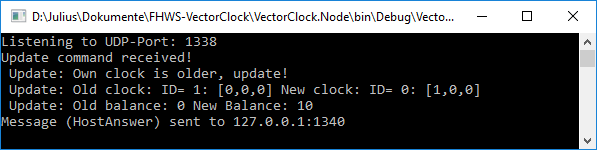
\includegraphics[width=10cm]{nodeWindow.png}
	\caption[Node Window]{Abbildung des Nodefensters. Zwischen den Nodes findet die eigentlichen Kommunikation statt.}
\label{figure:nodeWindow}
\end{figure}
\FloatBarrier

Die Kommunikation zwischen dem Commander und den Nodes wurde mittels UDP realisiert. Die Entscheidung viel auf UDP, da sich dadurch unnötiger Overhead und Programmieraufwand vermeiden lässt, welcher beispielsweise bei TCP angefallen wäre. Der Aufbau einer Nachricht ist in Abbildung \ref{Nachricht} dargestellt. Beim Absenden der Nachricht, egal ob im Commander oder in den Nodes, wird diese serialisiert und per UPD versendet. Im Empfangsfall muss der empfangene Datenstrom wieder deserialisiert und in eine Nachricht umgewandelt werden. 

TODO: Aufbau einer Nachricht darstellen
\cleardoublepage
\section{Schwierigkeiten von Vektoruhren}
\label{cap:problemeVC}
\subsection{Effizienten Speicherung von Vektoruhren}
% Paper: Concerning the size of clocks 
%        Plausible Clocks Constant Size Logical Clocks for Distributed Systems
Vektoruhren sind eine relativ einfache und effektive Lösung kausale Ordnung in einem verteilten System herzustellen.
Ihre Definition beherbergt jedoch ihren größten Nachteil.
Die Größe einer Uhr ist nicht konstant.
Für ein verteiltes System mit $n$ Prozessen benötigt eine Vektoruhr $n$ Komponenten i.d.R. Integer-Zahlen.
Die Folge ist, dass für ein großes verteiltes System alle Vektoruhren einen entsprechend hohen Speicherbedarf haben.
Dies wirkt sich zum einen negativ auf den Speicherverbrauch der einzelnen Prozesse aus, da je nach Implementierung mehrere Uhren gespeichert werden müssen.
Außerdem fügen die großen Vektoruhren einen Overhead zu den Nachrichten hinzu und belasten somit den Übertragungsweg.
Offensichtlich ist die Länge der Vektoruhr direkt proportional zur Anzahl der Prozesse.
Somit skalieren Vektoruhren schlecht \cite{torres1999plausible}.

Charron-Bost \cite{charron1990concerning} hat bewiesen, dass es innerhalb eines Systems bestehend aus $n$ Nodes immer eine mögliche Kombination an Ereignissen geben kann, bei der die Kausalität ausschließlich mit Vektoruhren der Länge $n$ erfasst werden kann.
Von daher müssen für alle theoretisch vorkommenden Prozesse innerhalb des Systems eine Komponente in der Uhr reserviert werden.
Dies beinhaltet alle aktuellen Prozesse und auch zukünftige Prozesse die möglicherweise ausgeführt werden könnten.
Es ist natürlich schwer im voraus zu entscheiden wie viele Prozesse potentiell ausgeführt werden und ist daher im Allgemeinen nur bei statischen Systemen gegeben, bei denen also  bei denen also die Anzahl der Prozesse konstant ist.
Daher muss theoretisch eine Vektoruhr mit einer statischen Länge von $n$ verwendet werden.
Im Folgenden werden verschiedene Verfahren vorgestellt um die Länge von Vektoruhren zu reduzieren.

Ein pragmatisches Vorgehen um die Länge einer Vektoruhr in einer annehmbarer Größe zu halten wurde von Amazon in ihrer Dynamo Datenbank \cite{decandia2007dynamo} verfolgt.
Hierbei wird die Länge durch folgendes Kürzungsschema reduziert:
Zu jeder Komponente in der Vektoruhr wird neben dem Zähler noch die Prozess ID und ein Zeitstempel gehalten.
Der Zeitstempel gibt den Zeitpunkt an, zudem der entsprechende Prozess zuletzt den Datensatz aktualisierte.
Erreicht die Länge der Vektoruhr einen bestimmten Schwellwert, werden die Komponenten mit den ältesten Zeitstempel aus der Uhr entfernt.
Dieses Verwerfen von Daten kann dazu führen, dass in gewissen Situationen die Kausalität nicht mehr komplett hergestellt werden kann.
Nach eigenen Angaben von \etal{DeCandia} \cite{decandia2007dynamo} trat dieses Problem im Produktiveinsatz jedoch nicht auf und wurde daher nicht weiter analysiert.

\etal{Singhal} \cite{singhal1992efficient} stellten ein einfaches Verfahren vor um den Overhead bei der Nachrichtenübertragung im Durchschnitt zu verringern.
Ihre Technik basiert auf der empirischen Beobachtung, dass nur wenige Prozesse häufig miteinander kommunizieren.
Außerdem ist es wahrscheinlich, dass zwischen zwei aufeinanderfolgend Sende-Ereignisse von Prozess $P_i$ zu $P_j$ nur wenige Komponenten der Vektoruhr sich ändern.
In diesem Fall ist es unnötig die komplette Uhr mit jeder ausgehenden Nachricht von $P_i$ zu $P_j$ zu übertragen.
Es ist ausreichend nur die Komponenten zu übertragen die sich geändert haben.
Konkret kann bei einer gegeben Uhr $VC$ für jede geänderte Komponenten ein Tupel aus $(a, VC[a])$ übertragen werden, wobei $a$ dem Index des Prozess innerhalb der Uhr entspricht.
Werden Vektoruhren nach dieser Technik übertragen kann die zu übertragene Datenmenge reduziert werden.
Dabei wird jedoch der lokale Speicherbedarf eines Prozesses erhöht, da dieser zusätzlich speichern muss welche Werte zuletzt zu welchen Prozess geschickt wurden.
Anhand den gespeicherten Vektoren kann er die entsprechenden Tupel auswählen, die an eine Nachricht mit angehängt werden müssen.

\begin{figure}[ht]
    \centering
    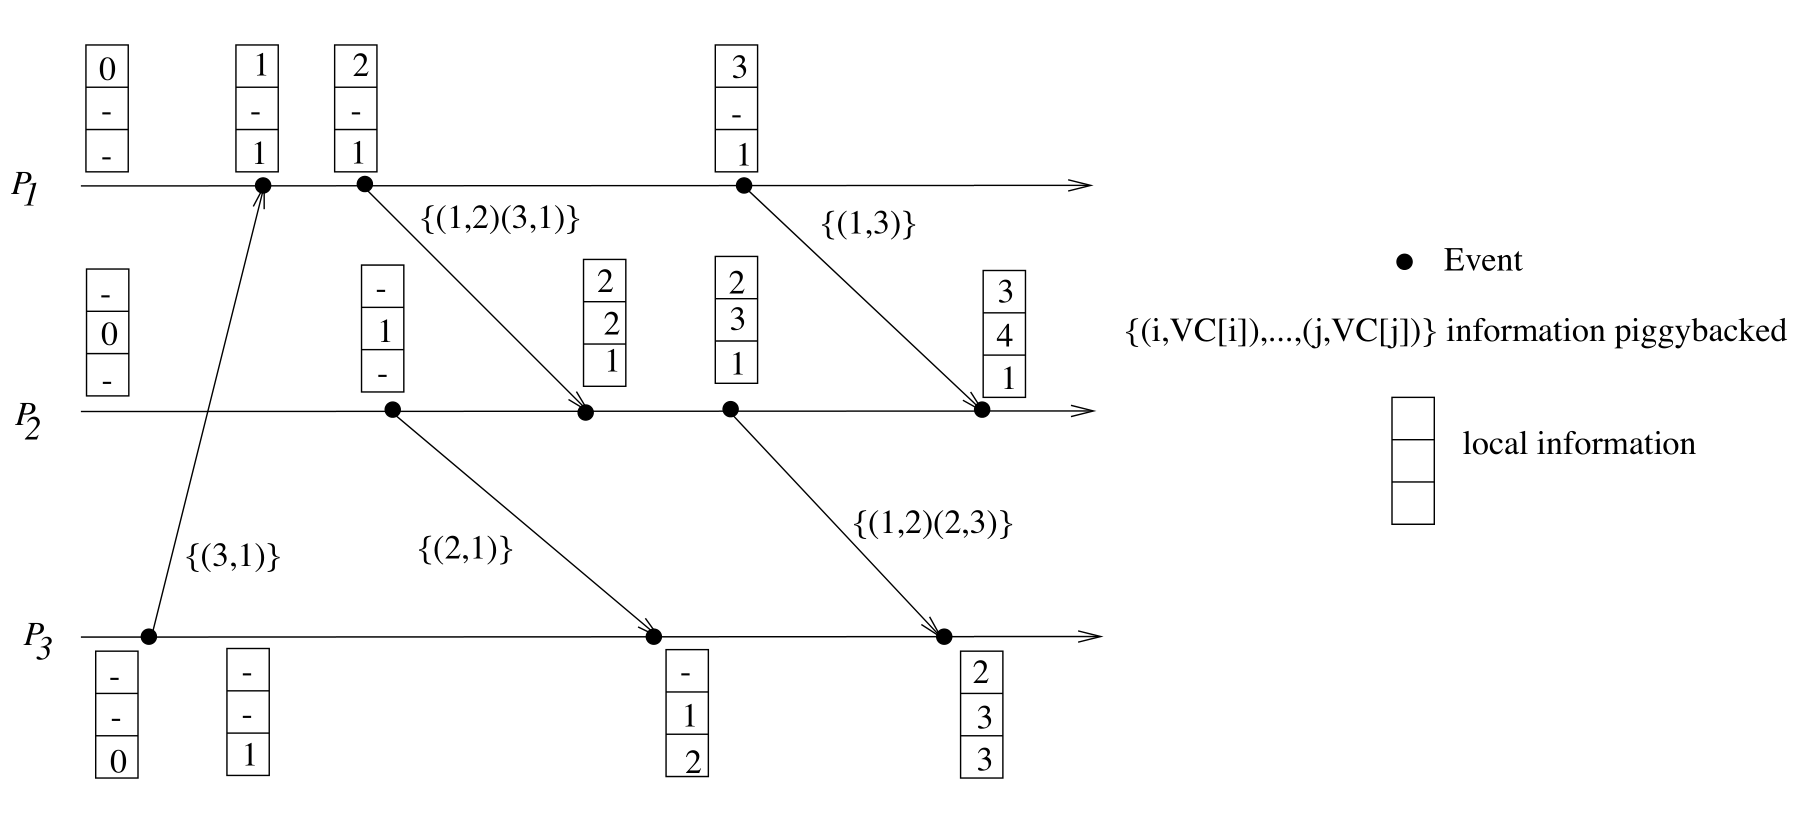
\includegraphics[width=1\textwidth]{Singhal.png}
    \caption[Kommunikaiton nach Singhal]{Ablauf der Kommunikation dreier Prozesse nach dem Verfahren von \etal{Singhal}.}
    Quelle: Nachgezeichnet aus \cite{Baldoni:2002:FDC:1435723.1437765}
    \label{fig:singhal}
\end{figure}

Bisher wurde immer angenommen, dass die Anzahl der Prozesse innerhalb eines Systems konstant ist.
Dies ist jedoch selten der Fall, in der Regel werden Prozesse häufig gestartet und beendet.
Die Folge ist, dass bei einer naiven Implementierung der Vektoruhr für jeden jemals ausgeführten Prozess eine Komponente in der Uhr reserviert werden muss.
In dynamischen Systemen kann dies dazu führen, dass die Uhren schnell eine tragbare Größe überschreiten.
Es ist daher wünschenswert Vektoruhren für solche dynamische Systeme zu optimieren.

Fridge \cite{fidge1991logical} stellte ein Modell vor bei dem eine variable Anzahl an Prozess-IDs verwendet wird.
Hierbei müssen die Prozess-IDs innerhalb des Systems eindeutig sein.
Beim Start eines Prozesses wird ihm eine ID zugewiesen.
Die ID eines terminierten Prozesses wird jedoch nicht freigegeben.
Damit die IDs solcher Prozesse freigegeben werden können, müssen allen anderen Prozesse die Terminierung bekannt sein.
Ist dies nicht gegeben, darf die ID nicht aus der Vektoruhr entfernt werden.
Diese Art von Garbage Collection wird in \cite{richard1998efficient} verwendet.
Alle Verfahren dieser Art haben jedoch das Problem, dass IDs von terminierten Prozessen nicht wiederverwendet werden können und die Bereinigung der Uhr von terminierten Prozessen durch einen einzigen unerreichbaren Prozess bereits verhindert werden kann \cite{almeida2008treeclocks}.

% Hier würde Landes reinpassen

Wie gezeigt führt die Verwendung von globalen IDs zu neuen Problemen.
Es liegt somit nahe auf globale IDs gänzlich zu verzichten.
Aus dieser Überlegung heraus entwickelten \etal{Almeida} \cite{almeida2008treeclocks} eine Generalisierung von Vektoruhren.
Die sogenannten \qq{Interval Tree Clocks} sind für dynamische Systeme ausgelegt und kommen dabei ohne globale IDs aus, indem jeder Prozess selbständig neue IDs erzeugen, löschen oder wiederverwenden kann, ohne das dabei auf eine globale Kommunikation zurückgegriffen werden muss.
Durch teilen und zusammenfassen von Prozess IDs wachsen und schrumpfen die Zeitstempel entsprechend zu der Dynamik des Systems.
Der Platzbedarf der Zeitstempel skaliert somit mit der Anzahl der Prozesse und wächst nur moderat an \cite{almeida2008treeclocks}.

% \cite{almeida2008treeclocks}
% landes dynamic clock

Ein in der Praxis relevantes Problem ist die Handhabung von Integer Überlaufen der Zählern innerhalb der Uhr.
In der Theorie werden die natürlichen Zahlen als Menge der möglichen Zählerwerte angenommen und haben somit keine Beschränkung.
Bei der Implementierung einer Vektoruhr muss jedoch über die Darstellung der Vektorkomponenten entschieden werden.
In der Regel wird ein Integer Datentyp mit typischerweise 32 oder 64 Bit gewählt.
Dabei muss ein Kompromiss zwischen maximale Länge und Datenmenge die zu übertragen ist gefunden werden.
Wird das verteilte System lange genug ausgeführt oder treten hochfrequent Ereignisse auf, kann es durchaus passieren, dass die Bitgrenze des gewählten Datentyps erreicht ist und ein Overflow zur Folge ist.
Dabei springt der Zähler vom Maximalwert auf Null.
\etal{Yen} \cite{yen1997resetting} stellen hierzu ein Protokoll vor um die Uhren zurückzusetzen.
Wird dieses Schema implementiert kann bei manche Anwendungen darauf verzichtet werden die optimale Bitlänge der Vektorkomponenten zu bestimmen. Da lediglich ein geeigneter Auslöser für den Uhrenreset gefunden werden muss \cite{yen1997resetting}.
Ein allgemeingültiges Verfahren wurde von Baldoni \cite{baldoni1998positive} vorgestellt.

% cap:vectorclock
\subsection{Gleichzeitig abgesendete Nachrichten}
\label{lbl:consistency}
% Verteiltes System
% Replika
% Konsitenz 
consistency

% Strong
>
Causal
>
Eventual

Wie bereits in der Einführung erwähnt, existiert kein globaler Zustand in einem verteilten System.
Vielmehr wird die Vereinigung aller lokalen Zustände als globaler Zustand verstanden.
Voraussetzung hierzu ist, dass alle Prozesse zu einem gewissen Zeitpunkt den selben lokalen Zustand haben.

Konkret kann es sich bei einem globalen Zustand zum Beispiel um ein Datenfeld in einer verteilten Key-Value-Datenbank handeln.
Jedes Datenfeld kann durch einen eindeutigen Schlüssel aus der Datenbank ausgelesen werden.
Alle Prozesse halten eine Replikation dieser Schlüssel-Werte Paare.
Durch die Kopie hat sich die Identität der Entität nicht geändert, das heißt obwohl eine Kopie gemacht wurde, handelt es sich immer noch um das selbe Objekt.

Wird nun in einem Prozess dieses Datenfeld modifiziert, muss die Änderung allen anderen Prozessen bekannt gemacht werden, damit diese den neuen Wert annehmen können.
Solange die Prozesse nach einer Datenänderung unterschiedliche Werte haben, ist das System inkonsistent, da je nachdem an welchem Prozess die Entität abgefragt wird, ein abweichender Wert zurück gegeben werden kann.
Der Umgang mit Änderungen und der Tolerierung eines solchen Zeitfensters, indem das System inkonsistent ist, führt zu einer Klassifizierung nach Konsistenzmodelle.

Es existieren eine Vielzahl an unterschiedlichen Modelle, die auf einer Skala von schwach nach strikt geordnet werden können.
Bei strikter Konsistenz (engl. \qq{strong consistency}) sind alle Replika immer identisch. Dies wird erreicht indem jedes Replika in der selben Reihenfolge aktualisiert wird und die Aktualisierung atomar durchgeführt wird.

Bei der Entwicklung einer verteilten Applikation aufbauend auf einer verteilten Datenbank mit strikter Konsistenz treten, im Vergleich zu einer herkömmlichen Datenbank, keine zusätzliche Schwierigkeiten auf.
Durch die strikte Konsistenz können keine Dateninkonsistenzen auftreten, ähnlich einer herkömmlichen relationalen Datenbank.
Gleichzeitig ist sie aber das teuerste Modell in der Umsetzung, da ein großer Kommunikationsaufwand betrieben werden muss.

Schwache Konsistenz (engl. \qq{weak consistency}) fordert, dass jedes Replika zu irgendeinen Zeitpunkt alle Aktualisierungen erhalten wird, ohne Forderungen an der Reihenfolge zu stellen.
Ein Applikation kann sich daher kaum auf die verteilte Datenbank verlassen, da durch die schwache Konsistenz kaum Versprechen über die Aktualität der Daten gemacht wird.
So kann eine spätere Aktualisierung eine frühere überschreiben, wenn ihre Nachricht schneller zugestellt wurde als die konkurrierende Nachricht.

Zwischen schwacher und strikter Konsistenz kann die sogenannte eventual consistency eingeordnet werden.
Ähnlich zur schwachen Konsistenz werden hier keine Leseinkonsistenzen eliminiert, zwei direkt aufeinander folgende Leseoperationen könne zwei unterschiedliche Werte ausgeben.
Es wird jedoch garantiert, dass sich das System stabilisieren und zu einem bestimmten Zeitpunkt alle Replika den selben Wert haben werden.
Die Aktualisierungen können in einer anderen Reihenfolge von einem Prozess empfangen werden, als sie gesendet wurden.
Der Prozess muss jedoch in der Lage sein die Aktualisierungen zu ordnen um den endgültigen Wert ohne Datenverlust zu bestimmen.

Einige verteilte System fordern nur sehr schwache Konsistenzbedingungen.
So ist die eventual consistency ein häufig implementiertes Konsistenzmodell.
Ein Beispiel für eine verteilte Datenbank die nach eventual consistency arbeitet ist Dynamo von Amazon \cite{decandia2007dynamo}.
Hier wird zu Gunsten der Geschwindigkeit auf eine strenge Konsistenz verzichtet.

Amazon setzt in ihrer Dynamo Datenbank Vektoruhren ein, um die Aktualisierungen in ihrer korrekten Ordnungen anzuwenden, wie es von eventual consistency gefordert ist.
Hierzu erhält jedes Objekt seine eigne Vektoruhr und fungiert als Version des Objekts.
Wird ein Replika verändert, inkrementiert es die Vektoruhr des Datenfeldes und teilt alle anderen Replika die Werteänderung mit.
Erhält ein Replika eine Aktualisierung zu der eine vorhergehende Aktualisierung noch nicht bei dem zu verarbeiteten Prozess angekommen ist, muss diese aufgeschoben werden.
Durch die Vektoruhr kann in den meisten Fällen bestimmt werden, welche Schreiboperation zuvor durchgeführt wurde.
In \fig{fig:vecConcurrent} ist eine solche aufgeschobene Aktualisierung dargestellt.

\begin{figure}[ht]
    \centering
    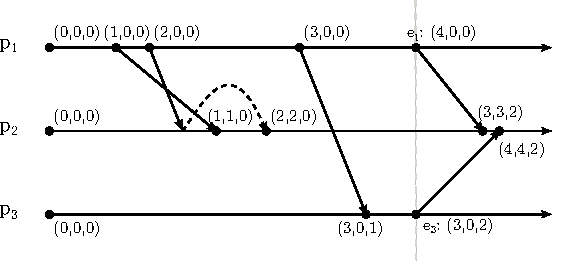
\includegraphics[width=1\textwidth]{VektorConcurr.pdf}
    \caption[Aufheben von Nachrichten]{Grafische Darstellung zweier Konflikte. Zum einen muss eine Nachricht richtig eingeordnet werden, da sie überholt wurde und zum anderem wurden die Nachrichten zu $e_1$ und $e_2$ gleichzeitig verschickt.}
    \label{fig:vecConcurrent}
\end{figure} 

Es kann jedoch passieren, dass durch die Vektoruhr keine Reihenfolge zwischen zwei Aktualisierungen festgestellt werden konnte, nämlich genau dann wenn $e_1 \parallel e_2$ gilt.
Diese nebenläufige Schreiboperationen, also Operationen die noch nicht abgeschlossen sind bevor Neue ausgeführt werden, stellen ein Problem für die eventual consistency dar.
Um einen Datenverlust zu vermeiden muss entschieden werden, in welcher Reihenfolge die Schreiboperationen ausgeführt werden sollen.
Die Schwierigkeit besteht jedoch darin, dass die Vektoruhr keine Aussage hierzu treffen kann.
\fig{fig:vecConcurrent} zeigt zwei gleichzeitig aufgetretene Schreiboperationen $e_1$ und $e_3$.
Durch die Vektoruhren kann auf die Nebenläufigkeit $e_1 \parallel e_3$ getestet werden:
\begin{align*}
      VC_3(e_3)[1] & \leq VC_1(e_1)[1] & \wedge & & VC_1(e_1)[3] & \leq VC_3(e_3)[3] \\
         3         & \leq 4            & \wedge & & 0            & \leq 2
\end{align*}

Da es sich hierbei um eine wahre Aussage handelt gilt, dass $e_1$ und $e_2$ gleichzeitig aufgetreten sein müssen.
Nun muss entschieden werden wie mit so einer Situation umgegangen wird.
Da die Middelware, die in der Regel die Handhabung der Vektoruhr übernimmt, keinerlei Informationen über den Inhalt der Datenfelder oder generell über die kommunizierten Daten hat, kann sie nur den Konflikt an die Applikationsschicht melden und eine Auflösung des Konflikts anfordern.
Wie die Applikation endgültig den Konflikt löst ist stark anwendungsabhängig und unterscheidet sich von Fall zu Fall.
Eine einfache, jedoch mit Datenverlust behaftete Lösung ist es die letzte Schreiboperation zu übernehmen und die ältere zu verwerfen.

Die Amazon Datenbank unterscheidet zwischen syntaktische und schematische Konflikte.
Können die Operationen durch die Vektoruhren kausal geordnet werden, gilt der Konflikt als syntaktisch gelöst.
Ist dies nicht möglich muss er schematisch gelöst werden, also durch die Applikationsschicht.


\subsection{Aufheben alter Nachrichten}
% 1. Ereignisse müssen alle Prozesse mitgeteilt werden. Nachrichten müssen solange aufgehoben werden, bis alle die Nachricht erhalten haben. Anhand von Nachrichten der anderen Prozessen kann mit deren Vektorclock entschieden werden welche Nachrichten sie von einem selbst schon haben
% 2. Nachrichten müssen für eventual Consitiency aufgehoben werden. Daei kann es passieren, dass eine Nachricht rein kommt die bereits die alten Zustände enthält und somit die alten Nachrichten obsolete.
% 3. Matrix Clock 'fire and forget'
% http://stackoverflow.com/questions/21359184/what-do-matrix-clocks-solve-but-vector-clocks-cant
% Voraussetzung: eventual consistency
% Zeigen Ohne Matrix würde es nicht gehen
% Matrix Uhren ermöglichen GC
Anhand Vektoruhren kann entschieden werden, wann zwischengespeicherte Nachrichten gelöscht werden können.
Hierzu gibt es drei potentielle Situationen in denen, entschieden werden muss wann etwas sicher gelöscht werden kann.
Für die ersten Beiden können Vektoruhren angewendet werden und für die letzte muss eine Erweiterung von Vektoruhren heran gezogen werden.

Eine Situation in der alte Nachrichten aufgehoben werden müssen, ist gegeben wenn ein Prozess seine versandet Nachrichten aufheben muss für den Fall, dass sie neu angefordert werden.
Andere Prozesse könnten unter gewissen Umständen Nachrichten erneut anfordern, wenn diese auf die Nachricht warten.
Eine andere Möglichkeit ist es, dass eine Synchronisation der Uhren angefordert wurde und die Prozesse sich versuchen anzugleichen.
Hierzu wird jede versandte Nachricht gespeichert, inklusive der Vektoruhr zum Zeitpunkt des Versendens.
Damit der Speicherbedarf nicht ins Unendliche wächst, müssen gespeicherte Nachrichten auch wieder gelöscht werden.
Dazu muss jedoch bekannt sein, welche Nachrichten gelöscht werden können ohne einen Datenverlust zu verursachen.

Eine Möglichkeit ist es, die Vektoruhren der eingehenden Nachrichten mit den Uhren der gespeicherten Nachrichten zu vergleichen.
Erhält der Prozess eine Vektoruhr eines anderen Prozesses indem seine Vektorkomponente größer oder gleich die der gespeicherten Nachricht ist, muss der andere Prozess die alten Nachricht bekommen und verarbeitet haben.
Dies ist durch die Updatevorschriften der Vektoruhr immer gegeben.

Verschickt der Prozess $i$ zu einem gegebenen Zeitpunkt $x$ seine Nachricht und speichert diese, muss der Empfänger $j$ das Maximum zwischen seiner lokalen Uhr und der Uhr aus der Nachricht für die Komponente des Prozesses $i$ nehmen.
Nun kann der Wert in der Nachricht das Maximum sein.
In diesem Fall wird der Zeitpunkt $x$ in die lokale Uhr übernommen.
Andernfalls hat der Empfänger bereits aktuellere Nachrichten von $i$ empfangen und seine lokale Vektoruhr erhält einen Wert $>x$.

In jedem Fall wird die zu dem Senderprozess zugehörige Komponente der Vektoruhr einen größeren oder gleichen Wert haben als die gesendete Nachricht.
Schickt nun der Empfänger seinerseits eine Nachricht an den ursprünglichen Sender $i$ muss er seine lokale Vektoruhr mit anfügen.
Anhand dieser kann der Prozess $i$ bestimmen, welche Nachrichten bereits von $j$ verarbeitet wurden, nämlich alle die kleiner oder gleich der Vektoruhr von $j$ für die $i$-te Komponente sind.

Dieses Vorgehen funktioniert auch indirekt zwischen mehr als zwei Prozessen.
\fig{fig:vectorPiggyback} zeigt eine solche Situation.
Prozess $p_1$ sendet zwei Nachricht $m_1$ und $m_2$ an $p_2$.
Anschließend schickt $p_2$ eine Nachricht $m_3$ an $p_3$.
Zu diesem Zeitpunkt kennt $p_3$ den aktuellsten Stand von $p_2$ und auch $p_1$, da diese zum Zeitpunkt des Verschickens von $m_2$ von $p_2$ bekannt war.
Schickt nun $p_3$ eine Nachricht an Prozess $p_1$, kann dieser aus der Vektoruhr erschließen, dass $p_3$ die Information von Nachricht $m_1$ erhalten hat.
Sendet nun $p_2$ noch eine Nachricht an $p_1$, kann $p_1$ erkennen, dass alle im Prozess den aktuellen Zustand kennt.
Somit kann $p_1$ die gespeicherten Nachrichten $m_1$ und $m_2$ verwerfen, da das gesamte System sie bereits erhalten hat.

\begin{figure}[ht]
    \centering
    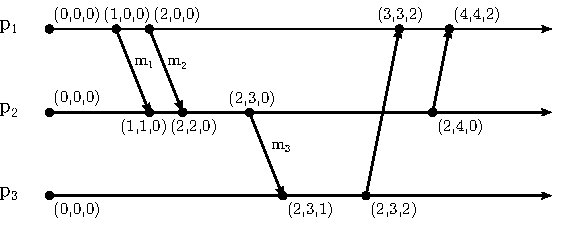
\includegraphics[width=1\textwidth]{VektorPiggypack.pdf}
    \caption[Löschen alter Nachrichten]{Am Ende der dargestellten Kommunikation kann  $p_1$ sowohl $m_1$ als auch $m_2$ verwerfen, da dem kompletten System die Information bekannt ist.}
    \label{fig:vectorPiggyback}
\end{figure} 

Eine zweite Situation in der alte Nachrichten, diesmal auf der Empfängerseite, gespeichert werden, ergibt sich wenn die Auslieferung der Nachrichten kausal geordnet erfolgen soll.
Dies ist zum Beispiel der Fall bei eventual consistency, da Aktualisierungen in der selben Reihenfolge angewendet werden muss in der sie aufgetreten sind.
Sendet nun ein Prozess $p_1$ Nachrichten an einen Prozess $p_2$, können diese in beliebiger Reihenfolge bei $p_2$ ankommen, dürfen jedoch nur in der Sendereihenfolge an die Applikation übertragen werden.

Nachrichten die außerhalb der Reihenfolge angekommen sind, müssen solange gespeichert werden bis die erwartete Nachricht ankommt.
Dies kann auch Nachrichten von einem dritten Prozess betreffen, da diese kausal von den restlichen Nachrichten abhängen können.
Sobald die erwartete Nachricht eingetroffen ist, kann diese zugestellt werden und alle gespeicherten Nachrichten die nun in der Reihenfolge als nächstes kommen.

Die gespeicherten Nachrichten werden in der Regel in einer Prioritätswarteschlange (engl. \qq{priority queue}) gespeichert.
Diese ist nach den Vektoruhren der Nachrichten sortiert und ermöglicht einen effizienten Zugriff auf die gespeicherten Nachrichten.

Im Allgemeinem muss die Anwendung entscheiden, wie sie auf den Inhalt der Nachrichten reagiert.
Damit die Anwendung richtig entscheiden kann, müssen alle Nachrichten zugestellt werden.
Ist dies nicht gegeben, ist nicht garantiert, dass die Anwendung in jeden Fall korrekt funktioniert.
Es gibt jedoch Anwendungsfälle, wie zum Beispiel verteilte Datenbanken, bei denen nur die letzte Aktualisierung von Relevanz ist.
In diesem Fall können alle gespeicherten Nachrichten verworfen werden, wenn eine aktuellere Nachricht empfangen wurde.
Dies stellt eine mögliche Optimierung dar, da nicht alle Nachrichten sondern nur eine, die Aktuellste, der Anwendung gemeldet werden muss.

\fig{TODO} zeigt eine Situation in der die zu erst verschickte Nachricht $m_1$ von $p_1$ von den beiden Nachrichten $m_2$ und $m_3$ überholt wurde und somit als letztes bei $p_2$ angekommen ist.
Eine Möglichkeit ist es nun, dass $p_2$ die Nachrichten $m_2$ und $m_3$ bis zum Empfangen von $m_1$ aufhebt und die Nachrichten in der korrekten Reihenfolge der Anwendung zustellt.
Alternativ könnte $p_2$ aber auch beim Empfangen von $m_2$ und $m_3$ diese direkt Zustellen und $m_1$ verwerfen, da bereits aktuellere Nachrichten empfangen wurden und der Inhalt von $m_1$ bereits bekannt oder obsolete ist.

% TODO figure

Der letzte Anwendungsfall ist Garbage Collection innerhalb des verteilten Systems.
Angenommen ein Prozess möchte eine Nachricht verschicken und deren Information sofort wieder verwerfen.
Natürlich darf die Information nur gelöscht werden, wenn alle Prozesse diese erhalten haben.
Dabei soll es keine Rolle spielen ob die Information direkt an alle Prozesse oder auch über Umwege indirekt verteilt wird.
Hierzu müsste der Prozess die Vektoruhren der anderen Prozesse kennen.
Dies verhält sich ähnlich zu dem ersten beschriebenen Anwendungsfall.

Ein Lösung für dieses Problem stellen Matrixuhren dar.
Vektoruhren können als Wissenstand interpretiert werden.
$VC_a(x)[i]$ beschreibt was der Prozess $a$ über den Prozess $i$ weiß, zu dem Zeitpunkt als $e$ eingetreten ist.
Es liegt nahe dieses Wissen über andere Prozesse leicht erweitert werden kann, indem eine höher dimensionale Struktur verwendet wird.
So kann der Vektor zu einer Matrix erweitert werden und als Liste von Vektoren betrachtet werden.
Durch $MC_a(x)[i,j]$ kann der Prozess $a$ erfahren, was der Prozess $i$ über Prozess $j$ weiß, zum Zeitpunkt $e$.
Diese Erweiterung wird nach ihrer Struktur als Matrixuhr bezeichnet.
Gilt nun zum Beispiel für alle $i$ das $MC_j(e)[i, j] > k$, kann nun der Prozess $j$ erschließen, dass jedem Prozess bekannt ist, dass sein aktueller Zustand größer $k$ ist.
Die Updateregeln von Matrixuhren verhalten sich ähnlich zu denen von Vektoruhren \cite{garg2005concurrent}.

In unserem oben gegebenen Szenario können nun Matrixuhren sinnvoll eingesetzt werden.
Angenommen die Nachricht wurde zu dem Zeitpunkt $MC[i][i]=k$ von Prozess $i$ verschickt, dann muss
\begin{equation*}
\forall j \colon MC[j][i] \geq k
\end{equation*}
erfüllt sein, damit $i$ die Nachricht löschen kann.
Die obige Bedingung impliziert, dass die $i$-te Komponente der Vektoruhren aller Prozesse $j$ größer oder gleich $k$ sind.
Somit hat sich die Information von Prozess $i$ durch das komplette System verteilt und kann somit gelöscht werden \cite{garg2005concurrent}.



\cleardoublepage
\section{Besonderheiten von Vektoruhren}

Nach Betrachtung der Funktionsweise von Vektoruhren sowie einer Beschreibung von besonderen Problemen, gibt es noch weiterführende Aspekte zu beachten. 
TODO: Mehr text hier! 
\subsection{Causaly Ordered Multicast}

In einem Verteilten System kann es recht schnell passieren, dass sich die Reihenfolge von gesendeten Broadcasts bei dem Empfänger und dem Sender unterscheiden. Dies führt in gewissen Fällen zu Problemen, wenn z.B. die Daten eines zweiten Broadcast von denen des ersten abhängen, es also eine temporale korrelation gibt. Um diesen Problem zu lösen, haben Kenneth P. Birman und Thomas A. Joseph in \cite{Birman:1987:RCP:7351.7478} den sogenannten Causal Brooadcast eingeführt, welcher auch als Causaly Ordered Multicast bezeichnet werden kann.

Wie in \cite{Birman:1987:RCP:7351.7478}[S. 52, Kapitel 3.3] beschrieben, kann es vorkommen, dass sich die Reihenfolge der gesendeten Nachrichten eines Senders und die Reihenfolge der empfangenen Nachrichten am Empfänger unterscheiden. Dies kann etwa durch Verzögerungen auf dem Übertragungsweg geschehen. Bei einem herkömmlichen Broadcast, welcher in einem System mit Vektoruhren abgesendet wird, ist kein Mechanismus vorgesehen, um eine eventuell für die Funktionsweise der Anwendung notwendige Reihenfolge der versendeten Nachrichten einzuhalten. Die Broadcast-Nachricht wird einfach an alle Teilnehmer versendet und nicht weiter beachtet.

Anders ist dies bei einem Causaly Orderen Multicast. Wie der Name bereit vermuten lässt, spielt hierbei die Ordnung der Multicasts nach deren Kausalität, also der Ursache eine Rolle. Die Ursache ist in diesem Fall das Verschicken des Broadcast am Sender. Somit werden bei einem Causal Broadcast die Nachrichten nach deren Reihenfolge des Versendens am Empfängerprozess geordnet. Um eine Rückantwort eines jeden Nodes an den Sender mit einer Empfangsbestätigung zu vermeiden, kann ein Causally Ordered Multicast auf Basis der Vektoruhren in den Empfängern umgesetzt werden. Durch die Vektoruhr kann ein Node entscheiden, ob er bei Empfang einer Nachricht alle Broadcast des entsprechenden Senders erhalten hat, die in der kausalen Vergangenheit dieses Broadcasts empfangen hat. Ist dies nicht der Fall, muss er die Nachricht in eine Warteliste setzten und diese erst annehmen, sobald alle in der Zwischenzeit passierten Broadcasts angekommen sind. Abbildung \ref{figure:causalbroadcast} verdeutlicht diese Funktionsweise genauer.

\begin{figure}[ht]
	\centering
	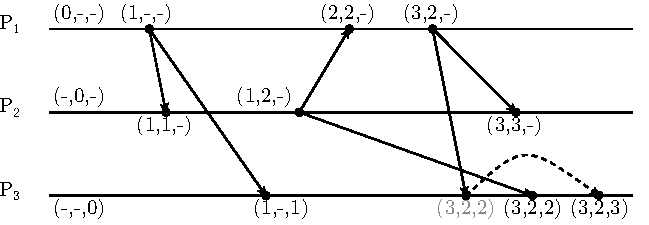
\includegraphics[width=10cm]{kommBeispielCausalBroadcast.pdf}
	\caption[Kommunikation durch Causally Ordered Multicasts]{Ablauf einer Kommunikation zwischen Prozessen, die ausschließlich Causally Ordered Multicasts versenden. Wie man sieht, muss ein Prozess eine Empfangene Nachricht aufheben, bis eine vorher gesendete Nachricht eintrifft.}
	\label{figure:causalbroadcast}
\end{figure}
\FloatBarrier

Der Ablauf des Aufhebens und Verzögerns von gewissen Nachrichten lässt sich durch ein recht einfaches Protokoll darstellen. Dieses ist in Abbildung \ref{figure:causalBroadcastProtocol} dargestellt.

\begin{figure}[ht]
	\centering
	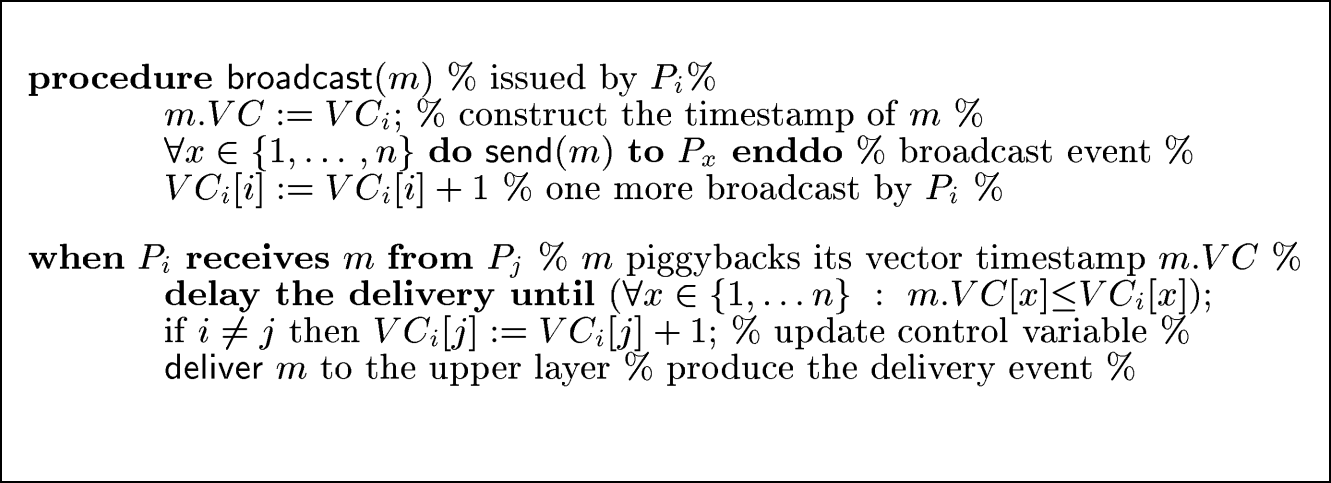
\includegraphics[width=10cm]{causalBroadcastProtocol.png}
	\caption[Protokoll für den Causally Ordered Multicast]{Beschreibung der verarbeitung von Causally Ordered Multicast in Form eines Protokolls.}
	Quelle: \cite{Baldoni:2002:FDC:1435723.1437765}[S. 7, Abbildung 3]
	\label{figure:causalBroadcastProtocol}
\end{figure}
\FloatBarrier

Ausgeschrieben sieht die Funktionalität des Protokolls folgendermaßen aus:

\begin{itemize}
	\item Löst ein Prozess durch ein stattgefundenes Event einen Broadcast aus, so fügt er zunächst seine aktuelle Vektoruhr an die Nachricht des Broadcasts an. Nun sendet er die Nachricht an alle teilnehmenden Prozesse und aktualisiert im letzten Schritt seinen Eintrag in der lokalen Vektoruhr.
	\item Empfängt ein Prozess $P_i$ eine Nachricht m des Prozesses $P_j$, so muss er die Nachricht so lange verzögern, bis die Bedingung $m.VC[x] \le VC_i[x]$ erfüllt ist, also bis die Nachricht ein direkter Nachfolger der Vorherigen ist. Anschließend wird der wert VC[j] inkrementiert, um das Sendeevent des Prozesses $P_j$ zu verzeichnen. Nun kann die Nachricht an die Anwendungsschicht weitergegeben werden.
\end{itemize}

Im Laufe der Kommunikation kann es passieren, dass mehrere nacheinander empfangenen Nachrichten nicht sofort verwendet sondern verzögert werden müssen. Für diesen Fall bietet es sich an, die verzögerten Nachrichten in einer liste zu speichern und bei Eintreffen einer Neuen Nachricht alle zunächst zurückgehaltenen nach deren \qq{alter} zu verarbeiten.

\subsubsection{Umsetzung in C\# auf Basis der Vektoruhr}
Causaly Ordered Multicasts wurden als Erweiterung der in Kapitel \ref{vectorClockImpl} beschriebenen Implementierung eingefügt. In dem gewählten Bank-Szenario sendet ein Bankautomat bei jeder Kontoaktualisierung, also einem Event, einen Broadcast an alle im System vorhandenen Prozesse. Dabei ist es jedoch egal ob die gesendeten Nachrichten über die Aktualisierung auch ankommen oder nicht beziehungsweise spielt die Reihenfolge des Empfangs für den Sender keine Rolle. Dieses System funktioniert solange, bis ein Prozess einmal eine Aktualisierung zu spät erhält und somit seinen Kontostand nicht entsprechend zum richtigen Zeitpunkt aktualisiert. Um diesem Problem entgegenzuwirken, können Causal Broadcasts helfen.

Als Grundlage dient die in Kapitel \ref{vectorClockImpl} implementierte Vektoruhren-Mechanik. Jedoch gibt es einige Unterschiede bei der Aktualisierung der Uhren beziehungsweise des Zeitpunkts der Aktualisierung.


 
\subsection{Rolle der Anwendungsschicht (Anwendungs-API)}

\cleardoublepage
\section{Abschließende Überlegungen}
\label{cap:schluss}
Dieses Kapitel schließt das Thema Vektoruhren dieser Arbeit ab. Neben einer Zusammenfassung der gesamten Arbeit einschließlich eines Fazits zu den einzelnen Themen wird ein Ausblick gegeben, wie man die Verwendung von Vektoruhren in einem Verteilten System noch verbessern und erweitern kann.
\subsection{Fazit}
In dieser Arbeit wurde zunächst beschrieben, wie ein Verteiltes System aufgebaut ist und welche Besonderheiten sich dabei ergeben. Nach einer Erklärung, weshalb es wichtig ist, Ausgetauschte Nachrichten in einem solchen System in eine gewisse kausale Ordnung zu bringen, fand eine Aufzählung der wichtigsten Uhrkonzepte statt. Neben den naheliegenden, physikalischen Uhren wurden die für das Thema dieser Arbeit interessanten logischen Uhren eingeführt und kurz deren Funktionsweise angeschnitten. Besonders hier hat sich bereits herausgestellt, dass Vektoruhren im Bereich der logischen Uhren sehr vielversprechende Funktionen bieten.

Nach der Einführung fand eine genauere Erklärung statt, wie Vektoruhren funktionieren. Diese wurde anhand von Beispielen näher erläutert und die Umsetzung in der Programmiersprache C\# präsentiert. Da sich bei dem Einsatz von Vektoruhren einigen Schwierigkeiten aufzeigen lassen, wurden einige davon in Kapitel Vier beschrieben. Hier wurden schnell die Grenzen der Uhren ersichtlich, nämlich dass Vektoruhren grundsätzlich nur bei statischen Systemen mit einer festen Anzahl an Prozessen funktionieren und die Größe der zu speichernden Uhren mit jedem weiteren Prozess stark zunimmt, was den gesamten Datenverkehr in die Höhe treibt. Auch machen Events, welche zum selben Zeitpunkt abgesendet werden, für eine reine Vektoruhr-Implementierung Probleme und lösen Konflikte aus.

Eine Besonderheit im Thema Vektoruhren stellt der Causally Ordered Multicast dar. Da dieser eine großen Mehrwert für die Anwendungsebene eines verteilten Systems haben kann, befasste sich der Autor in Kapitel 5 mit diesem Thema und ging auch hier wieder auf eine mögliche Umsetzung eines solchen Systems in C\# ein. Der Mehrwert bedeutet dabei, dass mit dieser Art des Multicasts Absendereihenfolgen von Absendern mit der Empfangsreihenfolge von Nachrichten an den Empfängern aufeinander abgestimmt werden können, was für viele Anwendungen von Großer Bedeutung sein kann. Als Beispiel wurde hierbei eine Aktualisierung von Kontoständen in einem Bankkonto-Szenario angeführt.

Neben den Eigenschaften des Causally Ordered Mulitcast wurde in diesem Kapitel zudem noch auf die besondere Rolle der Anwendungsschicht in einem verteilten System eingegangen. Wie sich herausstellte, macht eine kausale Ordnung von ankommenden Nachrichten erst im Kontext der Anwendung Sinn. So hängt es von dem tatsächlichen Anwendungsfall des verteilten Systems ab, ob zum Beispiel Nachrichten als zu löschend markiert werden können, wann alten Nachrichten tatsächlich gelöscht werden und welche Daten durch einen Prozess in einem Event verändert wurden. Im Sonderfall kann sich dadurch die Bedeutung von kausalen Zusammenhängen der ausgetauschten Nachrichten ändern.

Abschließend bleibt zu sagen, dass sich Vektoruhren sehr gut für die Ordnung und Sortierung von ausgetauschten Nachrichten in verteilten Systemen eignen. Durch Erweiterungen wie etwa dem Causally Ordered Multicasts kann dies sogar noch gezielter geschehen. Man darf jedoch nicht zu viel von der Funktionsweise der Uhren erwarten. Sie dienen lediglich als Basis und unterstützen die Anwendungsschicht dabei, sinnvoll mit ankommenden Nachrichten umzugehen und diese im Kontext des Anwendungsziels zu verarbeiten. Fehler auf dem Übertragungsweg oder der Ausfall von beteiligten Prozessen können durch Vektoruhren lediglich erkannt, jedoch nicht direkt verhindern oder ausgebessert werden. Dies bleibt weiterhin Aufgabe der Anwendungsebene.
\subsection{Ausblick}
Die grundlegende Funktionsweise von Vektoruhren ist bereits ein sehr interessantes und umfangreiches Thema. In der Literatur finden sich aufbauend darauf noch viele weitere Einsatzmöglichkeiten für diese Art der logischen Uhren.

Dabei lassen sich grundsätzlich zwei verschiedene Varianten unterscheiden. Die erste nimmt Vektoruhren als Basis und ändert deren Funktionalität derart ab, sodass damit ein spezielles Problem gelöst werden kann. Die zweite Variante nimmt Vektoruhren in der Funktionsweise, wie sie auch in dieser Arbeit beschrieben wurde und setzt sie für Anwendungen ein, die sich von der Ursprünglichen Idee der kausalen Ordnung von Nachrichten in verteilten Systemen unterscheidet. Im Folgenden werden für beide Fälle einige interessante Beispiele aus der Literatur gezeigt.

Die effiziente Speicherung von Vektoruhren ist, wie sich herausgestellt hat, in großen Systemen mit vielen beteiligten Prozessen ein Problem. Neben der in dieser Arbeit vorgestellten Lösung über Matrixuhren gibt es noch weitere, weitaus effizientere aber auch komplexere Ansätze für die Lösung dieses Problems. Eines davon sind die in \cite{Gidenstam2004} vorgestellten NUREV-Clocks, was ausgeschreiben für \textit{Non-Uniformly Mapped R-Entries Vector Clocks} steht. Die Idee dieser Art von Uhren ist es, eine dynamische Zuordnung zwischen den Prozessen in System und deren Einträgen in der Vektoruhr zu schaffen und dabei die Vektorgröße zu beschränken. Im herkömmlichen Fall ist diese starr, jeder Prozess hat also eine feste ID. Die Zuordnungen können während der Laufzeit dann dynamisch angepasst und optimiert werden, was im Endeffekt eine effizientere Speicherung und Übertragung der Vektoruhren während der Kommunikation ermöglicht.

Eine Anwendung, die in eine ähnliche Richtung geht wie NUREV-Clocks, sind \textit{Hierarchische Vektoruhren}. Diese spiele bei Systemen eine Rolle, welche aus physikalischen, geographischen oder administrativen Gründen zu einzelnen Gruppen aus Nodes zusammengefasst sind \cite{Khotimsky1999}[S. 1]. In diesen Systemen ist es wichtig, das Systemverhalten durch kausale Ordnung von Events im Hinblick auf Datenzugriffe, Konsistenzüberwachung und Fehlertoleranz zu überprüfen. Auch hier kommt wieder der Aspekt zum tragen, dass bei großen Systemen mit mehreren Hierarchieebenen der Speicheraufwand für Vektoruhren zur Überwachung sehr groß werden kann. \etal{Khotimsky} haben in  \cite{Khotimsky1999} eine hierarchische Vektoruhr entwickelt, welche über mehrere dieser Ebenen hinweg funktioniert und auf Basis der \textit{plausible logical time} arbeitet. Durch diese Art der Zeit kann ein Mittelweg zwischen Genauigkeit und den Kosten für einen Overhead gefunden werden, sie wurden in \cite{torres1999plausible} eingeführt und arbeiten unabhängig von der Anzahl an Nodes im System.

Ein etwas anderer Anwendungsfall ist eine Ordnung von Events in parallel arbeitenden Systemen. Diese arbeiten nicht verteilt, aber dafür mit mehreren, gleichzeitig ausgeführten Tasks. Im Programmablauf eines solchen Systems wechseln sich sequentielle und parallele Ausführungsschritte ab, was auch als \textit{Nested Parallelism} bezeichnet wird. Die in \cite{Audenaert1997} beschriebene Methode setzt dabei auf die Technik der \textit{Clock Trees}. Der Name wurde gewählt, weil sich im Laufe des Algorithmus eine Baumstruktur aus Vectoruhren bildet.


Für den zweiten Fall, also die Verwendung von Vektoruhren unter einem völlig neuen Kontext, lassen sich einige eher aktuelle, sehr auf serviceorientierte Architekturen und das Thema Social Media spezialisierte Anwendungen finden.
Ein erstes Beispiel hierfür ist das finden von Abhängigkeiten in Web-Services, wie es in \cite{Romano2011} durchgeführt wird. \etal{Romano} haben in ihrer Arbeit eine Methode entwickelt, wie man die Zusammenhänge unterschiedlicher, zusammenarbeitender Web-Services durch den Einsatz von Vektoruhren untersuchen kann. Das Problem bei solchen Systemen ist häufig, das dieses Zusammenspiel undurchsichtig ist und der Aufbau von serviceorientierte Architekturen schwer nachvollzogen werden kann. Eine direkte Folge stellt dabei die leichte Verbesserung der Antwortzeiten des in \cite{Romano2011} beschriebenen Systems durch eine solche Analyse und Anpassung dar.

Heutzutage sind Social-Media Plattformen wie Facebook oder Youtube in aller Munde. Durch die Vernetzung der User untereinander entstehen sehr große und komplexe Strukturen. Das gleiche Phänomen zeigt sich auch bei dem Emailaustausch innerhalb eines Unternehmens. Um die dynamischen Interaktionen und somit den Informationsfluss eines solchen Netzwerkes zu analysieren und darzustellen, können Vektoruhren verwendet werden. \etal{Hsu} \cite{Hsu2014} beschreiben eine Anwendung von Vektoruhren, welche sie als \textit{Variable Social Vector Clocks} benennen. Das Prinzip von \textit{Social Vector Clocks} wurde bereits in \cite{Kossinets2008} entwickelt und von \etal{Hsu} in dem Sinne erweitert, als dass auch unterschiedliche und damit dynamische Distanzen von Freundschaftsbeziehungen betrachtet werden. Dadurch können nicht nur direkte Freundschaften einbezogen werden, sondern auch indirekte über mehrere Freunde hinweg.

Wie man an diesen vielzähligen Beispielen sehen kann, eröffnete die Erfindung von logischen Uhren im allgemeinen und Vektoruhren im speziellen den Weg für viele interessante Weiterentwicklungen im Bereich der verteilten Systeme. Dieser Themenbereich ist auch heute noch sehr aktuell und nimmt mit zunehmender Digitalisierung der Unternehmen sogar noch an Bedeutung zu.


\clearpage
\printbibliography

\end{document}